\documentclass[cn,11pt,color=green,titlestyle=hang,mode=fancy,cite=numbers]{elegantbook}

\title{分数阶微积分}
\subtitle{Fractional Calculus}

\author{JiPan}
\institute{Harbin Institute of Technology}
\myemail{jipan\_2014@126.com}
\date{\today}
\version{V1.alpha.0.8}

\extrainfo{这书我没写过,不过确实在理 ——— ah Q LuXun}

\usepackage{makecell}
\usepackage{lipsum}
\usepackage{texnames}
\usepackage{amsmath,amsfonts}
\usepackage{mathrsfs}
\usepackage{booktabs}
\usepackage{cellspace}%
\setlength\cellspacetoplimit{3pt}
\setlength\cellspacebottomlimit{3pt}
\usepackage{makecell}
\usepackage{pgfplots}
\usepackage{tikz}

\usepackage{pstricks}
\usepackage{pstricks-add}
\usepackage{mathtools}

\setcellgapes{3pt}

\RequirePackage{amsmath}

\hfuzz=\maxdimen
\tolerance=10000
\hbadness=10000

\newcommand{\hint}[1]{\textbf{\textcolor[rgb]{1,0,0}{#1}}}
\newcommand{\under}[1]{\underline{#1}}
\newcommand{\chapterno}[1]{\chapter*{#1}  \addcontentsline{toc}{chapter}{#1}}
\newcommand{\vm}[1]{\textbf{\textit{#1}}}
\newcommand{\vmo}[1]{\overline{\textbf{\emph{#1}}}}

\logo{logo.png}
\cover{cover.jpg}

\begin{document}

	\maketitle

	\chapterno{序}
	\chapterno{前言}
	
	% \addcontentsline{toc}{chapter}{目\hspace{2em}录 }
	\tableofcontents

	\mainmatter
	\hypersetup{pageanchor=true}
	

	
	\chapterno{符号表}
	
	符号表、符号规定
	
	偶数空一页
	
	附录A
	
	参考文献
	
    重要字体颜色
	
	目录级别(三级)
	
	1.1.1.1
	
	\part{微积分基础(含线性代数、概率统计和实、复变函函数)}
	
		\chapter{初等数学}
		
		\chapter{微积分}
		
		\chapter{线性代数}
		
		\chapter{概率论}
		
		\chapter{统计学}
	
		\chapter{复变函数}

	\section{复数与复变函数}
	在本章中,首先结束复数系统的代数和几何结构。然后引进复变量的函数——复变函数,进而介绍他的连续性和连续性。
	
	\subsection{复数和四则运算}
	
	\subsubsection{复数的基本概念}
	为了便于后文说明,这里简单介绍复数的基本定义和结论。
	\begin{definition}{复数}{Complex number}
	设$x$和$y$为两实数,称形如
	\begin{equation}
	z =  x+\mathrm{i} y ~ (\mbox{或} x+y\mathrm{i})
	\end{equation}
	的数称为\hint{复数}。这里$\mathrm{i}$为虚数单位,具有性质$\mathrm{i}^2 = 1$,$x$和$y$分别称为复数$z$的实部和虚部。复数集记为$\mathbb{C}$,常记做
	$$ x = \mathrm{Re}\left(z\right),\quad y =  \mathrm{Im}\left(z\right).$$		
	\end{definition}
	虚部为零的数称为实数,简记为$x + \mathrm{i} 0 = x$,实数集记为$\mathbb{R}$。因此,全体实数为复数的一部分,特别的有
	$0 + \mathrm{i} 0 = 0$,即当且实部和虚部同时为零时$z$为零。当虚部不为零的复数称为\hint{虚数},而实部为零且虚部不为零的复数称为\hint{纯虚数}。如果量两复数的实部和虚部分别相等,则称两复数\hint{相等}。
	
	\subsubsection{复数的四则运算}
	\begin{theorem}{复数的四则运算}
		设$z_1$和$z_2$为两个复数
		$$z_1 =  x_1+\mathrm{i} y_1,\quad z_2 =  x_2+\mathrm{i} y_2.$$
		定义两复数$z_1$,$z_2$的四则运算为
		\begin{subequations}
			\renewcommand{\theequation}{\theparentequation-\arabic{equation}}
			\begin{align}  
			{}&z_1+z_2 = \left(x_1+\mathrm{i} y_1\right) +\left(x_2+\mathrm{i} y_2\right) = \left(x_1+x_2\right)+\mathrm{i}\left(y_1+y_2\right)                                   \label{eq:complex41} \\
			{}&z_1-z_2 = \left(x_1+\mathrm{i} y_1\right) -\left(x_2+\mathrm{i} y_2\right) = \left(x_1-x_2\right)+\mathrm{i}\left(y_1-y_2\right)                                  \label{eq:complex42} \\
			{}&z_1 \cdot z_2 = \left(x_1+\mathrm{i} y_1\right) \cdot \left(x_2+\mathrm{i} y_2\right) = \left(x_1x_2-y_1y_2\right)+\mathrm{i}\left(x_1y_2+y_1x_2\right)                                            \label{eq:complex43}
			\end{align}
			若$z_2 \ne 0$,则
			\begin{equation}
				\frac{z_1}{z_2} = \frac{x_1+\mathrm{i} y_1}{x_2+\mathrm{i} y_2} = \frac{\left(x_1+\mathrm{i} y_1\right)\left(x_2-\mathrm{i} y_2\right)}{\left(x_2+\mathrm{i} y_2\right)\left(x_2-\mathrm{i} y_2\right)} = \frac{x_1x_2+y_1y_2}{x^2_2+y^2_2} +\mathrm{i}\frac{x_2y_1-x_1y_2}{x^2_2+y^2_2}  \label{eq:complex44}
			\end{equation}
		\end{subequations}	
	\end{theorem}
	从式~\ref{eq:complex41}$\sim$式~\ref{eq:complex44} 可知复数经过四则运算仍然是复数,又从式~\ref{eq:complex41} 和式~\ref{eq:complex42} 以及虚部和实部的定义可知
	\begin{subequations}
		\renewcommand{\theequation}{\theparentequation-\arabic{equation}}
		\begin{align}  
			{}& \mathrm{Re}\left(z_1 \pm z_2\right) = \mathrm{Re}\left(z_1\right) \pm \mathrm{Re}\left(z_2\right) \label{eq:complex51} \\
			{}& \mathrm{Im}\left(z_1 \pm z_2\right) = \mathrm{Im}\left(z_1\right) \pm \mathrm{Re}\left(z_2\right) \label{eq:complex52} 
		\end{align}
	\end{subequations}

	\begin{example}
		\begin{enumerate}[noitemsep]
		\item 
		化简 $\displaystyle i^3,\frac{\mathrm{i}}{1-\mathrm{i}}+\frac{1-\mathrm{i}}{\mathrm{i}}. $
		\item 计算 (1)  $\displaystyle \frac{2+3\mathrm{i}}{2-3\mathrm{i}}$,\quad (2)  $\displaystyle \frac{2\mathrm{i}}{\sqrt{3}-\mathrm{i}}-\frac{3}{\sqrt{3}\mathrm{i}-1}$。
		\item 已知$x+y\mathrm{i} = \left(2x-1\right)+y^2\mathrm{i}$,求$z = x+\mathrm{i}y$。 
		\end{enumerate}
	\end{example}
	
	\begin{solution} 
		\begin{enumerate}[noitemsep]
			\item $\displaystyle -\mathrm{i},\quad -\frac{3}{2}-\frac{1}{2}\mathrm{i}$。
			\item (1) $\displaystyle -\frac{5}{13}+\frac{12}{13}\mathrm{i}$, \quad (2) $\displaystyle \frac{1}{4}+\frac{5\sqrt{3}}{4}\mathrm{i}$。
			\item $z = 1$ 或 $z = 1+\mathrm{i}$。
		\end{enumerate}
	\end{solution}

	\subsection{复数的几何表示}
	\subsubsection{复数的向量表示和复平面}
	任意给定的一个复数$z =  x+\mathrm{i}$,都有一对有序实数$\left(x,y\right)$相对应,而任意一对有序实数$\left(x,y\right)$都与直角坐标系$P\left(x,y\right)$对应。只有能够建立盘面上的全部点与全体复数简的一一对应关系,于是可用直角坐标系中的点来表示复数,如\figref{fig:vectorcomple}所示。
	
	\usetikzlibrary{angles}
	\usetikzlibrary{quotes}
	\begin{figure}[ht]
		\centering
		\begin{tikzpicture}[scale = 2]
		% \draw[step=1] (-0.5,-0.2) grid (4,3);
		\draw[-stealth,line width = 0.8pt] (-1.5,0) -- (4,0)node[below,scale=1]{$x$};
		\draw[-stealth,line width = 0.8pt] (0,-0.3) -- (0,3)node[right,scale=1]{$y$};
		\draw[-stealth,line width = 1pt,color = blue](0,0) -- (3,2.2);
		\draw[dashed,line width = 0.8pt,color = red](3,0) -- (3,2.2);
		\draw[dashed,line width = 0.8pt,color = red](0,2.2) -- (3,2.2);
		\node[below left] (n1) at (0.05, 0.05){$O$};
		\node[above right] (n2) at (2.95, 1.85){$P(x,y)$};
		\node[above right] (n3) at (2.75, 2.15){$z = x+ \mathrm{i}y$};
		\node[above left] (n4) at (1.5, 1){$r$};	
		\draw(2,0) coordinate (A) (0,0) coordinate (B) (3,2.2) coordinate (C) pic[draw,"$\theta$ ",line width = 1pt,angle eccentricity =1.2,-stealth,angle radius = 1cm]{angle};
		\end{tikzpicture}
		\caption{向量的几何表示}
		\label{fig:vectorcomple}
	\end{figure}
	
	表示复数$z$的直角坐标平面称为\hint{复平面}或 \hint{$z-$平面},复平面也常用集合$\mathbb{C}$来表示。因复平面上的$x$轴上的点对应实数,$y$轴上非零的点对应纯虚数,因此称$x$轴为实轴,$y$轴为虚轴。由于全体复数与复平面上的点的全体是一一对应的,以后吧“点$z$”和“复数$z$”作为同义词而不加以区别。
	
	在复平面上,如\figref{fig:vectorcomple}所示,从原点$O$到点$P\left(x,y\right)$作向量$\overrightarrow{OP}$。我们可以看到复平面上由原点$O$出发的向量的 全体和复数的全体$\mathbb{C}$之间也构成一一对应关系(复数$0$对应着零向量),因此也可以向量$\overrightarrow{OP}$来表示复数$z =  x+\mathrm{i}y$,其中$x$,$y$分别等于向量$\overrightarrow{OP}$沿$x$轴与$y$轴的分量。今后把“复数$z$”与其对应的向量$z$”也视为同义词。
	
	在物理学中,如力、速度、加速度等都可用向量表示,说明复数可以用来表示实有的物理量。
	
	\subsubsection{模与辐角}
	\begin{definition}{模与辐角}{abs and angle}
		向量$\overrightarrow{OP}$的长度$r$叫做复数$z$的\hint{模}或\hint{绝对值},记作$|z|$,即$|z| = r$。实轴正向转到与向量$\overrightarrow{OP}$方向一致时所成的角度叫做复数的\hint{辐角},记作$\mathrm{Arg} \left(z\right)$,即$\mathrm{Arg}\left(z\right)=\theta$。	
	\end{definition}
	
	复数$0$的模为零,即$|0|=0$,其辐角是不确定的。任何不为零的复数$z$的辐角$\mathrm{Arg} \left(z\right)$均有无穷多个值彼此之间相$2\pi$的整数倍通常把满足$-\pi < \theta \ne \pi$的辐角值$\theta_0$称为$\mathrm{Arg} \left(z\right)$的主值记为$\mathrm{arg} \left(z\right)$,于是
	\begin{equation}
	\mathrm{Arg} \left(z\right)=\mathrm{arg} \left(z\right)+ 2k\pi,\quad ,k=0,\pm1,\pm2,\cdots
	\end{equation}
	并且可以用复数$z$的实部来表示辅角的主值$\mathrm{arg} \left(z\right)$:
	\begin{equation}
	\arg z = \begin{dcases}
	  {\arctan \frac{y}{x},} & {x>0} \\
	  {\arctan \frac{y}{x}+\pi,} & {x>0, y>0} \\ 
	  {\arctan \frac{y}{x}-\pi,} & {x<0, y>0}\\
	  \end{dcases}
	\end{equation}
	
	由直角坐标与极坐标的关系(\figref{fig:vectorcomple}),我们立即得到不为零的复数的实部、虚部与该复数的模、辐角之间的关系
	\begin{equation}
	\left\{ 
	\begin{aligned}
	{}&r = |z| = \sqrt{x^2+y^2}\\
	{}&\tan\left(\theta\right) = \tan\left(	\mathrm{Arg} \left(z\right)\right) = \frac{y}{x}\\
	\end{aligned}
	\right. 
	\end{equation}
	
	以及
	\begin{equation}
	\left\{ 
	\begin{aligned}
	{}& x = z\cos \\
	{}&\tan\left(\theta\right) = \tan\left(	\mathrm{Arg} \left(z\right)\right) = \frac{y}{x}\\
	\end{aligned}
	\right. 
	\end{equation}
	
	于是复数z又可表示为
	
	a =r t	(cos0- ising	
	
	(1.2.3)式通常称为复数z的三角表示式如果再利用欧拉( Euler)公式
	
	
	我们又可以得到
	
	
	这种形式称为复数的指数表示式
	
	在§11节中已经指出:两复数的实部与虚部分别相等则称两复数相等.于
	
	是从(12.1)式与(122)式即知两复数相等,其模必定相等其辐角可以差2x的
	
	
	\begin{figure}[ht]
		\centering
		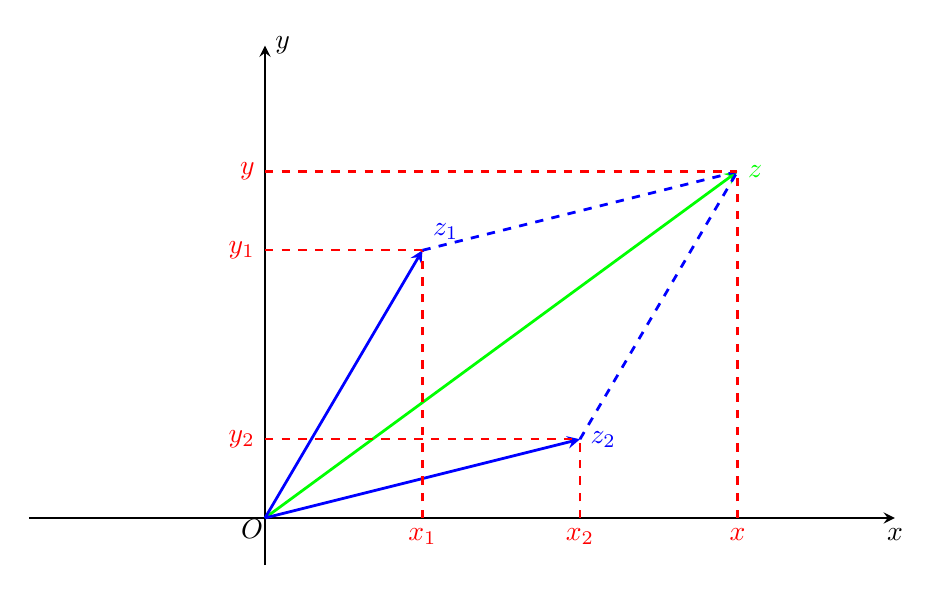
\begin{tikzpicture}[scale = 2]
		\draw[-stealth,line width = 0.8pt] (-1.5,0) -- (4,0)node[below,scale=1]{$x$};
		\draw[-stealth,line width = 0.8pt] (0,-0.3) -- (0,3)node[right,scale=1]{$y$};
		\draw[-stealth,line width = 1pt,color = green](0,0) -- (3,2.2)node[right,scale=1]{$z$};
		\draw[-stealth,line width = 1pt,color = blue](0,0) -- (2,0.5)node[right,scale=1]{$z_2$};
		\draw[dashed,line width = 0.8pt,color = red](2,0)node[below,scale=1]{$x_2$} -- (2,0.5);
		\draw[dashed,line width = 0.8pt,color = red](0,0.5)node[left,scale=1]{$y_2$}-- (2,0.5);
		\draw[-stealth,line width = 1pt,color = blue](0,0) -- (1,1.7)node[above right,scale=1]{$z_1$};
		\draw[dashed,line width = 0.8pt,color = red](0,1.7)node[left,scale=1]{$y_1$} -- (1,1.7);
		\draw[dashed,line width = 0.8pt,color = red](1,0)node[below,scale=1]{$x_1$}  -- (1,1.7);
		\draw[dashed,line width = 1pt,color = blue](2,0.5) -- (3,2.2);
		\draw[dashed,line width = 1pt,color = blue](1,1.7) -- (3,2.2);
		\draw[dashed,line width = 0.8pt,color = red](3,0)node[below,scale=1]{$x$} -- (3,2.2);
		\draw[dashed,line width = 0.8pt,color = red](0,2.2)node[left,scale=1]{$y$} -- (3,2.2);
		\node[below left] (n1) at (0.05, 0.05){$O$};
		\end{tikzpicture}
		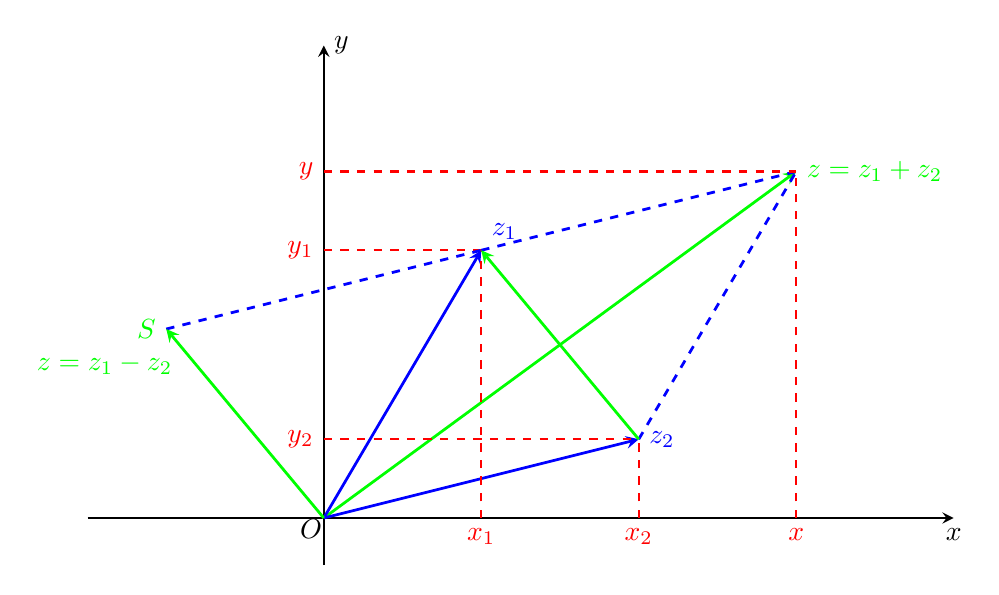
\begin{tikzpicture}[scale = 2]
		\draw[-stealth,line width = 0.8pt] (-1.5,0) -- (4,0)node[below,scale=1]{$x$};
		\draw[-stealth,line width = 0.8pt] (0,-0.3) -- (0,3)node[right,scale=1]{$y$};
		\draw[-stealth,line width = 1pt,color = green](0,0) -- (3,2.2)node[right,scale=1]{$z = z_1+z_2$};
		\draw[-stealth,line width = 1pt,color = blue](0,0) -- (2,0.5)node[right,scale=1]{$z_2$};
		\draw[dashed,line width = 0.8pt,color = red](2,0)node[below,scale=1]{$x_2$} -- (2,0.5);
		\draw[dashed,line width = 0.8pt,color = red](0,0.5)node[left,scale=1]{$y_2$}-- (2,0.5);
		\draw[-stealth,line width = 1pt,color = blue](0,0) -- (1,1.7)node[above right,scale=1]{$z_1$};
		\draw[dashed,line width = 0.8pt,color = red](0,1.7)node[left,scale=1]{$y_1$} -- (1,1.7);
		\draw[dashed,line width = 0.8pt,color = red](1,0)node[below,scale=1]{$x_1$}  -- (1,1.7);
		\draw[dashed,line width = 1pt,color = blue](2,0.5) -- (3,2.2);
		\draw[dashed,line width = 1pt,color = blue](1,1.7) -- (3,2.2);
		\draw[dashed,line width = 0.8pt,color = red](3,0)node[below,scale=1]{$x$} -- (3,2.2);
		\draw[dashed,line width = 0.8pt,color = red](0,2.2)node[left,scale=1]{$y$} -- (3,2.2);
		\node[below left] (n1) at (0.05, 0.05){$O$};
		\draw[-stealth,line width = 1pt,color = green](2,0.5) -- (1,1.7);
		\draw[dashed,line width = 1pt,color = blue](-1,1.2) -- (1,1.7);
		\draw[-stealth,line width = 1pt,color = green](0,0) -- (-1,1.2)node[left,scale=1]{$S$};
		\node[below left,color = green] (n1) at (-0.9,1.1){$z = z_1-z_2$};
		\end{tikzpicture}
		\caption{复数的加减法}
		\label{fig:complemp}
	\end{figure}

	\subsection{共轭复数}
	
	\subsection{复数的乘除、乘方和开方}
	
	\subsection{复球面与无穷远点}  % 复变函数
		
	\part{微分方程(含数理方程和特殊函数)}
	
    	%\chapter{常微分方程}

\begin{introduction}       
	\item 绪论
	\item 一阶常微分方程的初等解法
	\item 一阶常微分方程解得存在定理
	\item 高阶常微分方程 
	\item 一阶常微分方程组
	\item 非线性微分方程
	\item 一阶线性偏微分方程组		
\end{introduction}

\section{绪论}

若函数未知,但知道自变量、未知函数及函数的导数(或微分)组成的关系式,得到的便是\hint{微分方程},通过求解微分方求出未知函数。自变量只有一个的微分方程称为\hint{常微分方程},含有多个自变量的微分方程称为\hint{偏微分方程}。

\subsection{常微分方程模型}

\subsubsection{1.RLC电路}
$$
\frac{\mathrm{d^2}I(t)}{\mathrm{d}t^2}+\frac{R}{L}\frac{\mathrm{d}I(t)}{\mathrm{d}t}+\frac{I(t)}{LC} = \frac{1}{L}\frac{\mathrm{d}e(t)}{\mathrm{d}t}
$$

\subsubsection{2. 数学摆}
$$
\left\{ 
\begin{aligned}
{}&\frac{\mathrm{d^2}\varphi(t)}{\mathrm{d}t^2}+\frac{\mu}{m}\frac{\mathrm{d}\varphi(t)}{\mathrm{d}t}+\frac{g}{l}\sin(\varphi(t)) = \frac{1}{ml}F(t)\\
{}&\varphi(0) =\varphi_0\\
{}&\frac{\mathrm{d}\varphi(0)}{\mathrm{d}t}=\omega_0\\
\end{aligned}
\right. 
$$

\subsubsection{3.人口模型}

(1) Malthus:
$$
\left\{ 
\begin{aligned}
{}&\frac{N(t)}{\mathrm{d}t} = rN(t)\\
{}&N(t_0) = N_0\\
\end{aligned}
\right. 
$$

此微分方程的解为
$$
N(t) = N_0e^{r(t-t_0)}. 
$$

(2) Logistic:
$$
\left\{ 
\begin{aligned}
{}&\frac{N(t)}{\mathrm{d}t} = rN(t)(1-\frac{N(t)}{N_m})\\
{}&N(t_0) = N_0\\
\end{aligned}
\right. 
$$

此微分方程的解为
$$
N(t) = N_m\frac{e^{r(t-t_0)}N_0}{N_m-N_0+e^{r(t-t_0)}N_0}
$$

\subsubsection{4.传染病模型}

(1) SI模型
$$
\left\{ 
\begin{aligned}
{}&\frac{\mathrm{d}x(t)}{\mathrm{d}t} = ky(t)x(t)=kx(t)(n-x(t))\\
{}&x(0) = x_0\\
\end{aligned}
\right. 
$$

(2) SIS模型
$$
\left\{ 
\begin{aligned}
{}&\frac{\mathrm{d}x(t)}{\mathrm{d}t} = ky(t)x(t)-\mu x(t)=kx(t)(n-x(t)-\frac{\mu}{k})\\
{}&x(0) = x_0\\
\end{aligned}
\right. 
$$

(3) SIR模型
$$
\left\{ 
\begin{aligned}
{}&\frac{\mathrm{d}x(t)}{\mathrm{d}t} = ky(t)x(t)-\frac{\mathrm{d}r(t)}{\mathrm{d}t}=kx(t)y(t)-lx(t), \qquad& {} &  x(0) = x_0   \\
{}&\frac{\mathrm{d}y(t)}{\mathrm{d}t} = -kx(t)y(t), \qquad          & {} & y(0) = y_0 = n-x_0  \\
\end{aligned}
\right. 
$$

\subsubsection{5.两生物种群生态模型}

(1) Volterra被捕食-捕食模型$(a,b,c,d>0)$
$$
\left\{ 
\begin{aligned}
{}&\frac{\mathrm{d}x(t)}{\mathrm{d}t} = x(a-by)\\
{}&\frac{\mathrm{d}y(t)}{\mathrm{d}t} = y(-c+dx)\\
\end{aligned}
\right. 
$$

(2) 竞争模型$(a,b,c,d>0)$
$$
\left\{ 
\begin{aligned}
{}&\frac{\mathrm{d}x(t)}{\mathrm{d}t} = x(a-by)\\
{}&\frac{\mathrm{d}y(t)}{\mathrm{d}t} = y(c-dx)\\
\end{aligned}
\right. 
$$

(3) 共生模型$(a,b,c,d>0)$
$$
\left\{ 
\begin{aligned}
{}&\frac{\mathrm{d}x(t)}{\mathrm{d}t} = x(a+by)\\
{}&\frac{\mathrm{d}y(t)}{\mathrm{d}t} = y(c+dx)\\
\end{aligned}
\right. 
$$

(4) Volterra模型
$$
\left\{ 
\begin{aligned}
{}&\frac{\mathrm{d}x(t)}{\mathrm{d}t} = x(a+bx+cy) = M(x,y)x\\
{}&\frac{\mathrm{d}y(t)}{\mathrm{d}t} = y(d+ex+fy) = N(x,y)x\\
\end{aligned}
\right. 
$$

\subsubsection{6.Lorenz方程(分支和混沌)}
$$
\left\{ 
\begin{aligned}
{}&\frac{\mathrm{d}x(t)}{\mathrm{d}t} = a(y-x)\\
{}&\frac{\mathrm{d}y(t)}{\mathrm{d}t} = -xz+cx-y \\
{}&\frac{\mathrm{d}z(t)}{\mathrm{d}t} = xy-bz \\
\end{aligned}
\right. 
$$
其中参数为$a=10,b=8/3,c=28$

\subsubsection{7.化学动力学模型}

(1) Schlogt单分子化学动力学模型
$$
\frac{\mathrm{d}x}{\mathrm{d}t} = -k_3x^3+k_2Ax^2-k_1x+k_0B
$$

(2) 双分子化学动力学模型
$$
\left\{ 
\begin{aligned}
{}&\frac{\mathrm{d}x(t)}{\mathrm{d}t} = k_1Ax-k_2xy\\
{}&\frac{\mathrm{d}y(t)}{\mathrm{d}t} = k_2xy-k_3y\\
\end{aligned}
\right. 
$$

(3) 3分子化学动力学模型
$$
\left\{ 
\begin{aligned}
{}&\frac{\mathrm{d}x(t)}{\mathrm{d}t} = A-(B+1)X+x^2y\\
{}&\frac{\mathrm{d}y(t)}{\mathrm{d}t} = Bx-x^2y
\end{aligned}
\right. 
$$

\subsubsection{8.力学系统中的常微分方程模型}

(1) 牛顿力学
$$
\left\{ 
\begin{aligned}
{}& m \frac{\mathrm{d}\vec{r}}{\mathrm{d}t}=\vec{F}(t) \\
{}& J_c \frac{\mathrm{d}\vec{\theta}}{\mathrm{d}t} =\vec{M}(\vec{F}(t))  \\
\end{aligned}
\right. 
\left\{ 
\begin{aligned}
{}&m \frac{\mathrm{d}x(t)}{\mathrm{d}t} = F_x(t)\\
{}&m \frac{\mathrm{d}y(t)}{\mathrm{d}t} = F_x(t)\\
{}&J_c \frac{\mathrm{d}\theta_z(t)}{\mathrm{d}t} = M_c(\vec{F(t)})\\
\end{aligned}
\right. 
\left\{ 
\begin{aligned}
{}&m a_t = F_t(t)\\
{}&m a_n = F_n(t)\\
{}&J_c \frac{\mathrm{d}\theta_z(t)}{\mathrm{d}t} = M_c(\vec{F(t)})\\
\end{aligned}
\right. 
$$

(2) 拉格朗日力学

研究质点在三维欧氏空间中的运行,一个有势的牛顿力学系可以用质点的质量和力学系统的位能表达出来,牛顿运动方程使我们能完全解出一系列重要的力学问题。对有完整约束的力学系统,可以通过引进广义坐标($\varphi_1,\varphi_2,\cdots,\varphi_n$)接触约束,从而牛顿力学进行为拉格朗日力学。拉格朗日力学是利用一个拉格朗日函数$L(q_1,q_2 ,\cdots,q_n)$刻画系统,把力学系统的求解归结为在相应的坐标领域内求拉格朗日方程
$$
	\frac{\mathrm{d}}{\mathrm{d}t}\frac{\partial L}{\partial \dot{q}_i} -\frac{\partial L}{\partial q _i} = 0
$$

(3) 哈密顿力学

\subsection{基本概念和常微分方程的发展历史}

\section{一阶常微分方程的初等解法}
\section{一阶常微分方程解得存在定理}
\section{高阶常微分方程}
\section{一阶常微分方程组}
\section{非线性微分方程}
\section{一阶线性偏微分方程组}	  % 常微分方程
    	
    	%\chapter{分析力学基础}

\begin{introduction}   
	\item 虚位移原理
	\item 自由度和广义坐标
	\item 以广义坐标表示的质点系平衡条件 
	\item 动力学普遍方程
	\item 第二类拉格朗日方程
	\item 拉格朗日方程的初积分 
	\item 第一类拉格朗日方程	
\end{introduction}

18世纪提出了处理多个约束的刚体系统动力学问题。利用矢量力学分析出现以下问题:

(1)对于复杂约束系统约束力的性质和分布是未知的;

(2)表述形式复杂。如球坐标系下的运动方程;

(3)质点系问题为大量方程的微分方程组。            

1788年拉格朗日发表了《 分析力学》一书,提出了解决动力学问题的新观点和新方法:\hint{采用功和能量来描述物体的运动和相互作用力之间的关系}。

与矢量力学相比,分析力学的特点:    

(1)把约束看成对系统位置(速度)的限定,而不是看成一种力。

(2)使用广义坐标、功、能等标量研究系统运动,大量使用数学分析方法,得到标量方程。

(3)追求一般理论和一般模型,对于具体问题,只要代入和展开的工作,处理问题规范化。

(4)不仅研究获得运动微分方程的方法,也研究其求解的一般方法。

\section{虚位移原理}

\subsection{约束及其分类}

限制质点或质点系运动的条件称为\hint{约束}。限制条件的数学方程称为\hint{约束方程}。

(1)几何约束和运动约束:限制质点或质点系在空间的几何位置的条件称为几何约束。限制质点系运动情况的运动学条件称运动约束。

(2)定常约束和非定常约束:不随时间变化的约束称定常约束。约束条件随时间变化的称非定常约束。

(3)其它分类:约束方程中包含坐标对时间的导数,且不可能积分成有限形式的约束称非完整约束。约束方程中不包含坐标对时间的导数,或者约束方程中的积分项可以积分为有限形式的约束为完整约束。约束方程是等式的,称双侧约束(固执约束)。约束方程为不等式的,称单侧约束(非固执单侧约束)。

通常的约束为定常的双侧、完整、几何约束。即$n$个质点,$s$个约束。
$$f_i(x_1,y_1,z_1,\cdots,x_n,y_n,z_n) =0, \qquad i=1,2,\cdots s $$

\subsection{虚位移·虚功}

(1)虚位移:在某瞬时,质点系在约束允许的条件下,可能实现的任何无限小的位移称为虚位移。只与约束条件有关。通常表示为$\delta \vec{r}$,$\delta x$,$\delta \varphi$。

(2) 虚功:力在虚位移上作的功称虚功。
$$\delta W = \vec{F}\cdot \delta \vec{r} \qquad \delta W = M \delta \varphi$$
\subsection{理想约束}

如果在质点系的任何虚位移中,所有约束力所作虚功的和等于零,称这种约束为理想约束。即

$$\delta W_N = \sum \delta W_{Ni} = \Sigma \vec{F}_{Ni}\cdot \delta \vec{r}_i$$

光滑固定面约束、光滑铰链、无重刚杆,不可伸长的柔索、固定端等约束为理想约束。

\subsection{虚位移原理}

设质点系处于平衡,有
$${{\vec{F}}_{i}}+{{\vec{F}}_{\text{N}i}}=0 \qquad  {{\vec{F}}_{i}} \cdot \delta  {{\vec{r}}_{i}} +{{\vec{F}}_{\text{N}i}} \cdot \delta {{\vec{r}}_{i}}={{\vec{F}}_{i}} \cdot \delta  {{\vec{r}}_{i}} = 0 $$
或记为 $ \sum{\text{ }\!\!\delta\!\!\text{ }{{W}_{Fi}}}=0 $。此方程称虚功方程,其表达的原理称虚位移原理或虚功原理。

对于具有理想约束的质点系,其平衡的充分必要条件是:作用于质点系的所有主动力在任何虚位移中所作的虚功的和等于零。解析式为
$$\sum{\left( {{F}_{xi}}\text{ }\!\!\delta\!\!\text{ }{{x}_{i}}+{{F}_{yi}}\text{ }\!\!\delta\!\!\text{ }{{y}_{i}}+{{F}_{zi}}\text{ }\!\!\delta\!\!\text{ }{{z}_{i}} \right)=0}$$

\section{自由度和广义坐标}

\subsection{自由度}

\begin{definition}{Degree of Freedom}{int}
	在完整约束的条件下,确定质点系位置的\hint{独立参数}的数目,称为质点系的\hint{自由度数},简称\hint{自由度}。
\end{definition}

\begin{example}
	确定一个质点在空间的位置需3个独立的参量,自由质点为3个自由度。
\end{example}
\begin{example}	
	确定一个质点在平面的位置需2个独立的参量,平面自由质点为2个自由度。	
\end{example}
\begin{example}	
	质点$M$被限定只能在球面的上半部分,${{(x-a)}^{2}}+{{(y-b)}^{2}}+{{(z-c)}^{2}}={{R}^{2}}$,这样质点在空间中的位置就由两个独立参数所确定,即它的自由度数为2。
\end{example}  % 分析力学基础
    	
    	% \chapter{数理方程的基础理论}

\begin{introduction}   
	\item 矢量分析与场论
	\item 函数空间
	\item 线性微分算符
	\item 线性微分算符的本征值问题
	\item 广义函数
\end{introduction}

\section{矢量分析与场论}

\subsection{矢量分析}

\subsection{场论}

\subsection{哈密顿算子}

\subsection{正交坐标系}


\section{函数空间}


\subsection{度量空间与赋范线性空间}

\subsubsection{度量空间}
	
	矢量是线性代数中的基本概念,作为构成线性空间的元素。矢量具有类似于正常三维矢量的代数特性,即矢量具有加法和数乘两种运算,并且遵从相对应的运算法则。但是它并具有长度和方向的集合特征。因此这里作为数学抽象的线性空间也能附加上于三维矢量分析类似的直观的几何结果。为此首先引入距离的概念。	

	\begin{definition}{度量空间与度量函数}{def2-3-2-1}
		元素(称为\hint{点}) $x$,$y$,$z$,$\cdots$的非空集合$\mathscr{X}$称为\hint{度量空间}(或\hint{距离空间}),如果对于每一对元素$x,y,z$,存在与它们相联系的一个实数$d(x,y)$,满足下列三个条件
		\begin{enumerate}
			\item (对称性)元素A到B之间的距离等于元素B到A之间的距离。
			$$d(x,y) = d(y,x);$$
			\item (非负性)元素之间的距离大于等于0,若距离等于0则为相同元素。
			$$ d(x,y) \ge 0, \quad d(X,Y)=0 \Leftrightarrow x=y;$$
			\item  (三角形不等式)元素之间的距离满足三角形不等式。
			$$d(x,y) \le d(x,z)+d(y,z).$$
		\end{enumerate}
		或可以理解为一个度量空间(metric space)由一个有序对(ordered pair) $(\mathscr{X},d)$ 表示,其中$\mathscr{X}$是一种集合
		,$d$是定义在$(\mathscr{X},d)$上的一种度量,是如下的一种函数映射:
		$$ \mathscr{X} \times \mathscr{X} \rightarrow \mathbb{R}.$$
		其满足上述三条性质,则称$(\mathscr{X},d)$度量空间或距离空间。$\mathscr{X}$中的元素称为点,点$P_0$的$\delta$邻域和点$P_0$的$\delta$去心邻域为
		\begin{equation}
		U(P_0,\delta) = \left\{P|d(P,P_0)<\delta \right\},\quad \stackrel{\circ}{U}(P_0,\delta) = \left\{P|0<d(P,P_0)<\delta \right\},
		\end{equation}	
		点$P_0$为邻域的中心,$\delta$称为邻域的半径。
	\end{definition}

	\begin{note}
		\begin{enumerate}
			\item 度量空间的元素(点)可以不是矢量。距离不仅仅是点与点之间的距离,除此之外还有向量之间的距离,曲线之间的距离,函数之间的距。这儿谈到距离的定义是一种泛指的概念。
			\item 无需定义元素的加法和数乘运算,因此度量空间可以不是线性空间,换言之,线性空间是度量空间的子集。
		\end{enumerate}
	\end{note}

	\begin{example}
		常见的度量空间如下:
		\begin{enumerate}
		\item 
			所有实数的集合(实轴)构成度量空间(记为$\mathscr{R}_1$),如果两个实数(实轴上的两点)$x$和$y$之间的距离定义为$|x-y|$.
		\item 
			所有复数$z = x+iy$的集合构成度量空间(记为$\mathscr{C}_1$),若两个复数$z_1$和$z_2$之间的距离定义为
			$$ d(z_1,z_2) = |z_1-z_2| = \sqrt{(x_1-x_2)^2+(y_1-y_2)^2}.$$
			\item 所有$n(n\in \mathbb{N^+})$个有序实数构成度量空间为$n$维欧式空间,记为$\mathscr{A}^{(r)}_{n}$。令
			$$x = (\xi_1,\xi_2,\cdots,\xi_n), \quad y = (\eta_1,\eta_2,\cdots,\eta_n)$$
			是空间中的两个点,引入不同的距离定义,就得到不同的度量空间,例如,可以定义距离函数为
			\begin{equation}
				d_p(x,y) = (|\xi_1-\eta_1|^p+|\xi_2-\eta_2|^p+\cdots+|\xi_n-\eta_n|^p)^{\frac{1}{p}} = [\sum_{i=1}^{n}(|xi_i-\eta_i|^p]^{\frac{1}{p}},\quad 1\le p\le \infty
			\end{equation}
			包括了取 $p = 1,2,\infty$的情形分别为直线距离,折线距离和最大距离:
			\begin{equation}
			\left\{  
			\begin{aligned}
			{}&d_1(x,y) = |\xi_1-\eta_1|+|\xi_2-\eta_2|+\cdots+|\xi_n-\eta_n| = \sum_{i=1}^{n}|\xi_i-\eta_i|\\
			{}&d_2(x,y) = (|\xi_1-\eta_1|^2+|\xi_2-\eta_2|^2+\cdots+|\xi_n-\eta_n|^2)^{\frac{1}{2}} = [\sum_{i=1}^{n}|\xi_i-\eta_i|^2]^{\frac{1}{2}}\\
			{}&d_\infty(x,y) = \max_i|\xi_i-\eta_i|\\
			\end{aligned}
			\right. 
			\end{equation}
		\item 
			所有$n(n\in \mathbb{N^+})$个有序复数构成度量空间为$n$维复空间,记为$\mathscr{A}^{(c)}_{n}$。
		\item 设$(\mathscr{X},d)$为度量空间,对$\mathscr{X}$中的任意两元素$x,y \in \mathscr{X}$,令
				\begin{equation}
					d(x,y)  = \left\{ 
					\begin{aligned}
					{}&1,\quad {\rm if ~}  x \neq y\\
					{}&0,\quad {\rm if ~}  x = y\\
					\end{aligned}
					\right. 
				\end{equation}
			这样的度量空间$(\mathscr{X},d)$称为离散的度量空间。
		\item 设$\mathcal{S}$为表示为实数列(复数列)的全体,对$\mathcal{S}$中任意两元素$x$,$y$
			$$x = (\xi_1,\xi_2,\cdots,\xi_n,\cdots), \quad y = (\eta_1,\eta_2,\cdots,\eta_n,\cdots)$$
			\begin{equation}
			d(x,y)  = \sum_{i=1}^{\infty} \frac{1}{2^i}\frac{|\xi_i-\eta_i|}{1+|\xi_i-\eta_i|}
			\end{equation}
			这样的度量空间$(\mathcal{S},d)$称为序列空间。
		\item
			设$\mathcal{A}$是一个给定的集合,令$\mathcal{B}(\mathcal{A})$表示$\mathcal{A}$上有界实值(或复值)函数全体,对$\mathcal{B}(\mathcal{A})$中任意两点$x$,$y$,定义
			\begin{equation}
				d(x, y)=\sup _{t \in \mathcal{A}}|x(t)-y(t)|
			\end{equation}
			这样的度量空间$(\mathcal{B}(\mathcal{A}),d)$称为有界函数空间。
		\item
			设$\mathcal{M}$为$\mathcal{X}$上实值(或复值)的勒贝格可测函数全体,$m$为勒贝格测度,若$m(X)<\infty$,对任意两个可测函数$f(t)$及$g(t)$,由于$ \displaystyle \frac{|f(t)-g(t)|}{1+|f(t)-g(t)|}<1 $,所以这就是$\mathcal{X}$上的可积函数。定义
			\begin{equation}
				d(f, g)= \int_{\mathcal{X}}\frac{|f(t)-g(t)|}{1+|f(t)-g(t)|}dt
			\end{equation}
		\item
			令$C[a,b]$表示闭区间$[a,b]$上实值(或复值)连续函数全体,对$C[a,b]$中任意两点$x$,$y$,定义
			\begin{equation}
				d(x, y)=  \max_{a\le t \le b} |x(t)-y(t)|
			\end{equation}
			这样的度量空间$(C[a,b],d)$称为$C[a,b]$空间。
		\item
			令$l^p$为集合$\displaystyle l^p =\{ x = (x_1,x_2,\cdots,x_i,\cdots ) |\sum_{i=1}^{\infty}x^p_k < \infty \}$,其中$x$,$y$为$l^p$中的两个元素,定义
			\begin{equation}
			d(x,y) = [\sum_{i=1}^{n}(|x_i-y_i|^p]^{\frac{1}{p}}
			\end{equation}
			这样的度量空间$l^p$空间。
		\end{enumerate}
	\end{example}

\subsubsection{度量空间中的极限、稠密集、可分空间}

	\begin{definition}{收敛点列}{def2-3-2-2}
		设$\{x_k\}$ 是$(\mathcal{X},d)$中的点列,如果任给$\epsilon>0$,存在指标$N$,使得
		$$d(x,x_k) \le \varepsilon, \quad  \forall k\le N \Leftrightarrow \lim _{k \rightarrow \infty} d\left(x_{k}, x\right)=0$$
		则称点列$\{x_k\}$是$(\mathcal{X},d)$中的\hint{收敛点列},点列$\{x_k\}$收敛到$x$ $(x_k \rightarrow x )$,或称$\{x_k\}$的极限为$x$,记为$\displaystyle \lim _{k \rightarrow \infty} x_{k}=x$。
	\end{definition}

	\begin{property}\label{property:converge_series}
		收敛点列的性质
		\begin{enumerate}
			\item 在度量空间中,任何一个点列最多只有一个极限,即收敛点列的极限是唯一的。
			\item $\mathcal{M}$是闭集的充要条件是$\mathcal{M}$中任何收敛点列的极限都在M中。
		\end{enumerate}
	\end{property}

	\begin{example}
		常见的度量空间的极限如下:
		\begin{enumerate}
			\item $n$维欧式空间中,$\{x_m\}$按欧式距离收敛于的充要条件是$x_m$依坐标收敛$x$,其中$x_m = (\xi_1^{(m)},\xi_2^{(m)},\cdots,\xi_n^{(m)})$,其中$m=1,2,\cdots$为$\mathbb{R}$的点列,$x = (\xi_1^{(m)},\xi_2^{(m)},\cdots,\xi_n^{(m)})$为点列$\{x_m\}$极限,则
			$$\lim _{m \rightarrow \infty} d\left(x_{m}, x\right)=0 \Leftrightarrow \lim _{m \rightarrow \infty} x_{m}=x \Leftrightarrow \lim _{m \rightarrow \infty} \xi ^{(m)}_i= \xi_i,i=1,2,\cdots m.$$
			\item 在序列空间序列$\mathcal{S}$中,$x_m = (\xi_1^{(m)},\xi_2^{(m)},\cdots,\xi_n^{(m)})$,其中$ m=1,2,\cdots$,序列$\{x_m\}$极限为$x = (\xi_1^{(m)},\xi_2^{(m)},\cdots,\xi_n^{(m)}) \in \mathcal{S} $,则
			$$\lim _{m \rightarrow \infty} d\left(x_{m}, x\right)=0 \Leftrightarrow \lim _{m \rightarrow \infty} x_{m}=x \Leftrightarrow \lim _{m \rightarrow \infty} \xi ^{(m)}_i= \xi_i,i=1,2,\cdots m.$$
			\item 设$\{ x_n\}$及$x$分别为$C[a,b]$中的点列及点,$d(x_m, x)=  \max_{a\le t \le b} |x_m(t)-x(t)|$,则
			$$\lim _{m \rightarrow \infty} d\left(x_{m}, x\right)=0 \Leftrightarrow \{x_n\} \mbox{在} [a,b] \mbox{上一致收敛于} x.$$
			\item 设$\{f_n\}$及$f$分别为可测函数空间中的点列及点,则
			$$\lim _{m \rightarrow \infty} d\left(f_{m}, x\right)=0 \Leftrightarrow \lim _{m \rightarrow \infty} f_n(t)= f(t).$$
		\end{enumerate}
	\end{example}
	
	\begin{definition}{有界集}{def2-3-2-3}
		设$\mathcal{M}$是度量空间$(\mathcal{X},d)$中点集,定义$\delta(\mathcal{M}) = \sup _{x,y \in \mathcal{X}} d(x,y)$为点集$\mathcal{M}$的直径,若$\delta(\mathcal{M}) <\infty$,则称$\mathcal{M}$为$(\mathcal{X},d)$中的有界集。度量空间中的收敛点列是\hint{有界点集}。	
	\end{definition}

	\begin{definition}{稠密集}{def2-3-2-4}
		设$\mathcal{X}$是度量空间,$\mathcal{E}$和$\mathcal{M}$是$\mathcal{X}$中的两个子集,令$\overline{\mathcal{M}}$表示$\mathcal{M}$的闭包,如果,$\mathcal{E} \subset \overline{\mathcal{M}}$,那么称集$\mathcal{M}$在集$\mathcal{E}$中\hint{稠密}。即如果$\mathcal{E}$中任何一点$x$的任何邻域都含有集$\mathcal{M}$中的点,就称$\mathcal{M}$在$\mathcal{E}$中稠密。
	\end{definition}


	\begin{note}
		\begin{enumerate}
			\item (\hint{稠密集的极限})对任一$x \in \mathcal{E}$,有$\mathcal{M}$中的点列$\{x_k\}$,使得$\displaystyle \lim _{k \rightarrow \infty} x_{k}=x$.
			\item (\hint{稠密子集})当$\mathcal{E}=\mathcal{X}$时,称集$\mathcal{M}$为$\mathcal{X}$的一个稠密子集。
			\item (\hint{可分空间}) 如果$\mathcal{X}$有一个可数的稠密子集时,称$\mathcal{X}$为可分空间。
		\end{enumerate}
	\end{note}

	\begin{example}
		常见的稠密集如下
		\begin{enumerate}
			\item 多项式全体所成的线性空间$\mathcal{P}$是度量空间$C[a,b]$ 的子集,则$\mathcal{P}$在$C[a,b]$ 中是稠密的。其中,以有理数为系数的多项式全体是一个可数集,所以$C[a,b]$是可分空间。
			\item $n$ 维欧式空间$\mathbb{R}^n$是可分空间,因为坐标为有理数的全体是一个可数集,是$\mathbb{R}^n$中的稠密子集。
			\item $l^p$为可分空间。$l^\infty$为不可分空间。
			令$l^p$为集合
			$$\displaystyle l^p =\{ x = (x_1,x_2,\cdots,x_i,\cdots ) |\sum_{i=1}^{\infty}x^p_k < \infty \}$$
			其中$x$,$y$为$l^p$中的两个元素,定义
			\begin{equation}
			d(x,y) = [\sum_{i=1}^{n}(|x_i-y_i|^p]^{\frac{1}{p}}
			\end{equation}
			这样的度量空间$l^p$空间。
		\end{enumerate}
	\end{example}

\subsubsection{连续映射}

	\begin{definition}{度量空间中的连续性}{def2-3-2-5}
		设$(\mathcal{X},d)$和$(\mathcal{Y},\tilde{d})$是两个度量空间,$T$是$\mathcal{X}$到$\mathcal{Y}$中的映射,$x_0 \in \mathcal{X}$ ,如果对于任意给定$\varepsilon>0$,存在$\delta>0$,使对$\mathcal{X}$中一切满足$d(x,x_0)<\delta$的$x$,有$\tilde{d}(Tx,Tx_0)<\varepsilon$成立,则称$T$在$x_0$处连续。	
	\end{definition}

	使用$\varepsilon-\delta$语言表述度量空间中的连续性为:
	$$T \mbox{ 在 }x_0\mbox{ 处连续 }\Leftrightarrow \forall U (Tx_0,\varepsilon)\mbox{ 必有 } V(x_0,\delta),\mbox{ 使得 } TV \in U.$$
	
	连续性定义也可以通过度量空间的极限进行定义。设$T$是度量空间$(\mathcal{X},d)$和$(\mathcal{Y},\tilde{d})$的映射,那么$T$在$x_0 \in \mathcal{X}$连续的充要条件为当$\displaystyle \lim _{k \rightarrow \infty} x_{k}=x_0$时,必有$\displaystyle \lim _{k \rightarrow \infty} Tx_{k}=Tx_0$。显示在度量空间在$x_0 \in \mathcal{X}$有极限是度量空间在$x_0 \in \mathcal{X}$连续的必要不充分条件。

	\begin{definition}{连续映射}{def2-3-2-6}
		如果映射$T$在$\mathcal{X}$的每一点都连续,则称$T$是$\mathcal{X}$上的连续映射。称集合$\{x | x \in X, T x \in M \subset Y\}$为集合$\mathcal{M}$在映射$T$下的原像。
	\end{definition}

	\begin{theorem}{连续映射的充要条件}{theo2-3-2-1}
	度量空间$\mathcal{X}$到$\mathcal{Y}$的映射T是$\mathcal{X}$上的连续映射的充要条件为$\mathcal{Y}$中任意开集$\mathcal{M}$的原像$T^{-1}M$ 是$\mathcal{X}$中的开集。
	\end{theorem}

\subsubsection{柯西点列和完备度量空间}


欧几里得空间,希尔伯特空间,巴拿赫空间或者是拓扑空间都属于函数空间。函数空间 = 元素 + 规则 ,即一个函数空间由 元素 与 元素所满足的规则 定义,而要明白这些函数空间的定义首先得从距离,范数,内积,完备性等基本概念说起。

二.范数
$$
范数 是比 距离 限制条件更多的一个概念。为了形象地解释范数的概念,这儿在二维平面进行说明。
在定义了 距离 这个概念之后,我们便可以描述二维平面上两个点之间的 距离 ,此时这个空间称作 度量空间 。但目前的条件没有办法描述一个点的“长度” ,因为缺少了 零点 。而范数定义之后此空间便多了一个零点,可以联想我们熟悉的平面直角坐标系,二维平面中范数可以看做是平面中的点到零点的距离。拥有范数的空间称作赋范空间,用符号∣∣X∣∣ ||X||∣∣X∣∣表示元素X XX的范数。因为范数的概念是在距离的概念上加了新的限制,则赋范空间一定是度量空间。我们可以用范数定义距离:
d(X,Y)=∣∣X−Y∣∣ d(X,Y)=||X-Y||
d(X,Y)=∣∣X−Y∣∣
$$
总结:元素X XX的范数∣∣X∣∣ ||X||∣∣X∣∣可简单看做X XX到零点的近距离。

三.线性
线性这个概念可以说是很熟悉了,即为加法与乘法的结合。若一个空间为线性空间,只要我们知道了此空间的所有基,便可以用加法与数乘表示这一空间所有的元素,如二维平面中能用X轴的单位向量与Y轴的单位向量表示此平面的任意向量。

$$
四.内积
内积又称点积或者数量积,在高中学习向量的点乘运算时便接触到这一概念。在有了前面的定义之后的空间总觉得与我们最熟悉的空间还差点什么,没错,就是角度。在引入内积之后的空间便有了角度的概念。X XX与Y YY的内积用符号(X,Y) (X,Y)(X,Y)表示,内积的结果同样是为实数。内积是在范数的概念上加了更多限制条件,即内积空间一定为赋范空间,同样的,可以用内积定义范数如下:
∣∣X∣∣2=(X,X) ||X||^2 = (X,X)
∣∣X∣∣ 
2
=(X,X)
$$

目前为止便完成了本文的大部分内容,有限维内积空间便是我们最熟悉的欧几里得空间。


$$
五.完备性
完备性这个概念的历史渊源比较深厚,作为非数学专业的工科生我也不太明白完备性的具体含义,简单来说对集合中的元素取极限不超出此空间便称其具有完备性。可以反向地通过不完备来理解完备性,对于整数集而言,对5取极限,便会超出整数集,即整数集不完备。
2018-10-22更正: 最近学了一点泛函,对完备性有了新的理解。完备性是在极限的基础上衍生的概念。例如在有理数集上的一个序列{1,1.4,1.41,1.414,1.4142…},可知此序列极限为2–√ \sqrt{2} 
2	
,而2–√ \sqrt{2} 
2	
为无理数,不属于有理数集,即有理数集不具备完备性。
$$

有了以上的概念理解众多迷糊人的空间便容易得多了

线性完备内积空间称作希尔伯特空间
线性完备赋范空间称作巴拿赫空间
有限维线性内积空间称作欧几里得空间
需要更加深入地理解希尔伯特空间大概避不开泛函分析,但作为工科学生,大概了解其概念够用就好。

线性空间

欧式空间

希尔伯特空间

\url{https://blog.csdn.net/qq\_34099953/article/details/84190508}

\url{http://open.163.com/movie/2013/3/T/0/M8PTB0GHI_M8PTBUHT0.html}  % 数理方程的基础理论
    	 
    	
	\part{微分方程数值解法}
	
    	%\chapter{常微分方程}

\begin{introduction}       
	\item 绪论
	\item 一阶常微分方程的初等解法
	\item 一阶常微分方程解得存在定理
	\item 高阶常微分方程 
	\item 一阶常微分方程组
	\item 非线性微分方程
	\item 一阶线性偏微分方程组		
\end{introduction}

\section{绪论}

若函数未知,但知道自变量、未知函数及函数的导数(或微分)组成的关系式,得到的便是\hint{微分方程},通过求解微分方求出未知函数。自变量只有一个的微分方程称为\hint{常微分方程},含有多个自变量的微分方程称为\hint{偏微分方程}。

\subsection{常微分方程模型}

\subsubsection{1.RLC电路}
$$
\frac{\mathrm{d^2}I(t)}{\mathrm{d}t^2}+\frac{R}{L}\frac{\mathrm{d}I(t)}{\mathrm{d}t}+\frac{I(t)}{LC} = \frac{1}{L}\frac{\mathrm{d}e(t)}{\mathrm{d}t}
$$

\subsubsection{2. 数学摆}
$$
\left\{ 
\begin{aligned}
{}&\frac{\mathrm{d^2}\varphi(t)}{\mathrm{d}t^2}+\frac{\mu}{m}\frac{\mathrm{d}\varphi(t)}{\mathrm{d}t}+\frac{g}{l}\sin(\varphi(t)) = \frac{1}{ml}F(t)\\
{}&\varphi(0) =\varphi_0\\
{}&\frac{\mathrm{d}\varphi(0)}{\mathrm{d}t}=\omega_0\\
\end{aligned}
\right. 
$$

\subsubsection{3.人口模型}

(1) Malthus:
$$
\left\{ 
\begin{aligned}
{}&\frac{N(t)}{\mathrm{d}t} = rN(t)\\
{}&N(t_0) = N_0\\
\end{aligned}
\right. 
$$

此微分方程的解为
$$
N(t) = N_0e^{r(t-t_0)}. 
$$

(2) Logistic:
$$
\left\{ 
\begin{aligned}
{}&\frac{N(t)}{\mathrm{d}t} = rN(t)(1-\frac{N(t)}{N_m})\\
{}&N(t_0) = N_0\\
\end{aligned}
\right. 
$$

此微分方程的解为
$$
N(t) = N_m\frac{e^{r(t-t_0)}N_0}{N_m-N_0+e^{r(t-t_0)}N_0}
$$

\subsubsection{4.传染病模型}

(1) SI模型
$$
\left\{ 
\begin{aligned}
{}&\frac{\mathrm{d}x(t)}{\mathrm{d}t} = ky(t)x(t)=kx(t)(n-x(t))\\
{}&x(0) = x_0\\
\end{aligned}
\right. 
$$

(2) SIS模型
$$
\left\{ 
\begin{aligned}
{}&\frac{\mathrm{d}x(t)}{\mathrm{d}t} = ky(t)x(t)-\mu x(t)=kx(t)(n-x(t)-\frac{\mu}{k})\\
{}&x(0) = x_0\\
\end{aligned}
\right. 
$$

(3) SIR模型
$$
\left\{ 
\begin{aligned}
{}&\frac{\mathrm{d}x(t)}{\mathrm{d}t} = ky(t)x(t)-\frac{\mathrm{d}r(t)}{\mathrm{d}t}=kx(t)y(t)-lx(t), \qquad& {} &  x(0) = x_0   \\
{}&\frac{\mathrm{d}y(t)}{\mathrm{d}t} = -kx(t)y(t), \qquad          & {} & y(0) = y_0 = n-x_0  \\
\end{aligned}
\right. 
$$

\subsubsection{5.两生物种群生态模型}

(1) Volterra被捕食-捕食模型$(a,b,c,d>0)$
$$
\left\{ 
\begin{aligned}
{}&\frac{\mathrm{d}x(t)}{\mathrm{d}t} = x(a-by)\\
{}&\frac{\mathrm{d}y(t)}{\mathrm{d}t} = y(-c+dx)\\
\end{aligned}
\right. 
$$

(2) 竞争模型$(a,b,c,d>0)$
$$
\left\{ 
\begin{aligned}
{}&\frac{\mathrm{d}x(t)}{\mathrm{d}t} = x(a-by)\\
{}&\frac{\mathrm{d}y(t)}{\mathrm{d}t} = y(c-dx)\\
\end{aligned}
\right. 
$$

(3) 共生模型$(a,b,c,d>0)$
$$
\left\{ 
\begin{aligned}
{}&\frac{\mathrm{d}x(t)}{\mathrm{d}t} = x(a+by)\\
{}&\frac{\mathrm{d}y(t)}{\mathrm{d}t} = y(c+dx)\\
\end{aligned}
\right. 
$$

(4) Volterra模型
$$
\left\{ 
\begin{aligned}
{}&\frac{\mathrm{d}x(t)}{\mathrm{d}t} = x(a+bx+cy) = M(x,y)x\\
{}&\frac{\mathrm{d}y(t)}{\mathrm{d}t} = y(d+ex+fy) = N(x,y)x\\
\end{aligned}
\right. 
$$

\subsubsection{6.Lorenz方程(分支和混沌)}
$$
\left\{ 
\begin{aligned}
{}&\frac{\mathrm{d}x(t)}{\mathrm{d}t} = a(y-x)\\
{}&\frac{\mathrm{d}y(t)}{\mathrm{d}t} = -xz+cx-y \\
{}&\frac{\mathrm{d}z(t)}{\mathrm{d}t} = xy-bz \\
\end{aligned}
\right. 
$$
其中参数为$a=10,b=8/3,c=28$

\subsubsection{7.化学动力学模型}

(1) Schlogt单分子化学动力学模型
$$
\frac{\mathrm{d}x}{\mathrm{d}t} = -k_3x^3+k_2Ax^2-k_1x+k_0B
$$

(2) 双分子化学动力学模型
$$
\left\{ 
\begin{aligned}
{}&\frac{\mathrm{d}x(t)}{\mathrm{d}t} = k_1Ax-k_2xy\\
{}&\frac{\mathrm{d}y(t)}{\mathrm{d}t} = k_2xy-k_3y\\
\end{aligned}
\right. 
$$

(3) 3分子化学动力学模型
$$
\left\{ 
\begin{aligned}
{}&\frac{\mathrm{d}x(t)}{\mathrm{d}t} = A-(B+1)X+x^2y\\
{}&\frac{\mathrm{d}y(t)}{\mathrm{d}t} = Bx-x^2y
\end{aligned}
\right. 
$$

\subsubsection{8.力学系统中的常微分方程模型}

(1) 牛顿力学
$$
\left\{ 
\begin{aligned}
{}& m \frac{\mathrm{d}\vec{r}}{\mathrm{d}t}=\vec{F}(t) \\
{}& J_c \frac{\mathrm{d}\vec{\theta}}{\mathrm{d}t} =\vec{M}(\vec{F}(t))  \\
\end{aligned}
\right. 
\left\{ 
\begin{aligned}
{}&m \frac{\mathrm{d}x(t)}{\mathrm{d}t} = F_x(t)\\
{}&m \frac{\mathrm{d}y(t)}{\mathrm{d}t} = F_x(t)\\
{}&J_c \frac{\mathrm{d}\theta_z(t)}{\mathrm{d}t} = M_c(\vec{F(t)})\\
\end{aligned}
\right. 
\left\{ 
\begin{aligned}
{}&m a_t = F_t(t)\\
{}&m a_n = F_n(t)\\
{}&J_c \frac{\mathrm{d}\theta_z(t)}{\mathrm{d}t} = M_c(\vec{F(t)})\\
\end{aligned}
\right. 
$$

(2) 拉格朗日力学

研究质点在三维欧氏空间中的运行,一个有势的牛顿力学系可以用质点的质量和力学系统的位能表达出来,牛顿运动方程使我们能完全解出一系列重要的力学问题。对有完整约束的力学系统,可以通过引进广义坐标($\varphi_1,\varphi_2,\cdots,\varphi_n$)接触约束,从而牛顿力学进行为拉格朗日力学。拉格朗日力学是利用一个拉格朗日函数$L(q_1,q_2 ,\cdots,q_n)$刻画系统,把力学系统的求解归结为在相应的坐标领域内求拉格朗日方程
$$
	\frac{\mathrm{d}}{\mathrm{d}t}\frac{\partial L}{\partial \dot{q}_i} -\frac{\partial L}{\partial q _i} = 0
$$

(3) 哈密顿力学

\subsection{基本概念和常微分方程的发展历史}

\section{一阶常微分方程的初等解法}
\section{一阶常微分方程解得存在定理}
\section{高阶常微分方程}
\section{一阶常微分方程组}
\section{非线性微分方程}
\section{一阶线性偏微分方程组}	  % 有限差分法
    	
		\chapter{有限体积法}
		
		\chapter{有限元法}

		\chapter{谱方法}
		
		\chapter{小波变换}
		
		\chapter{其他方法}
			\section{蒙特卡洛方法}
				
	\part{分数阶微分}
		%  \chapter{常微分方程}

\begin{introduction}       
	\item 绪论
	\item 一阶常微分方程的初等解法
	\item 一阶常微分方程解得存在定理
	\item 高阶常微分方程 
	\item 一阶常微分方程组
	\item 非线性微分方程
	\item 一阶线性偏微分方程组		
\end{introduction}

\section{绪论}

若函数未知,但知道自变量、未知函数及函数的导数(或微分)组成的关系式,得到的便是\hint{微分方程},通过求解微分方求出未知函数。自变量只有一个的微分方程称为\hint{常微分方程},含有多个自变量的微分方程称为\hint{偏微分方程}。

\subsection{常微分方程模型}

\subsubsection{1.RLC电路}
$$
\frac{\mathrm{d^2}I(t)}{\mathrm{d}t^2}+\frac{R}{L}\frac{\mathrm{d}I(t)}{\mathrm{d}t}+\frac{I(t)}{LC} = \frac{1}{L}\frac{\mathrm{d}e(t)}{\mathrm{d}t}
$$

\subsubsection{2. 数学摆}
$$
\left\{ 
\begin{aligned}
{}&\frac{\mathrm{d^2}\varphi(t)}{\mathrm{d}t^2}+\frac{\mu}{m}\frac{\mathrm{d}\varphi(t)}{\mathrm{d}t}+\frac{g}{l}\sin(\varphi(t)) = \frac{1}{ml}F(t)\\
{}&\varphi(0) =\varphi_0\\
{}&\frac{\mathrm{d}\varphi(0)}{\mathrm{d}t}=\omega_0\\
\end{aligned}
\right. 
$$

\subsubsection{3.人口模型}

(1) Malthus:
$$
\left\{ 
\begin{aligned}
{}&\frac{N(t)}{\mathrm{d}t} = rN(t)\\
{}&N(t_0) = N_0\\
\end{aligned}
\right. 
$$

此微分方程的解为
$$
N(t) = N_0e^{r(t-t_0)}. 
$$

(2) Logistic:
$$
\left\{ 
\begin{aligned}
{}&\frac{N(t)}{\mathrm{d}t} = rN(t)(1-\frac{N(t)}{N_m})\\
{}&N(t_0) = N_0\\
\end{aligned}
\right. 
$$

此微分方程的解为
$$
N(t) = N_m\frac{e^{r(t-t_0)}N_0}{N_m-N_0+e^{r(t-t_0)}N_0}
$$

\subsubsection{4.传染病模型}

(1) SI模型
$$
\left\{ 
\begin{aligned}
{}&\frac{\mathrm{d}x(t)}{\mathrm{d}t} = ky(t)x(t)=kx(t)(n-x(t))\\
{}&x(0) = x_0\\
\end{aligned}
\right. 
$$

(2) SIS模型
$$
\left\{ 
\begin{aligned}
{}&\frac{\mathrm{d}x(t)}{\mathrm{d}t} = ky(t)x(t)-\mu x(t)=kx(t)(n-x(t)-\frac{\mu}{k})\\
{}&x(0) = x_0\\
\end{aligned}
\right. 
$$

(3) SIR模型
$$
\left\{ 
\begin{aligned}
{}&\frac{\mathrm{d}x(t)}{\mathrm{d}t} = ky(t)x(t)-\frac{\mathrm{d}r(t)}{\mathrm{d}t}=kx(t)y(t)-lx(t), \qquad& {} &  x(0) = x_0   \\
{}&\frac{\mathrm{d}y(t)}{\mathrm{d}t} = -kx(t)y(t), \qquad          & {} & y(0) = y_0 = n-x_0  \\
\end{aligned}
\right. 
$$

\subsubsection{5.两生物种群生态模型}

(1) Volterra被捕食-捕食模型$(a,b,c,d>0)$
$$
\left\{ 
\begin{aligned}
{}&\frac{\mathrm{d}x(t)}{\mathrm{d}t} = x(a-by)\\
{}&\frac{\mathrm{d}y(t)}{\mathrm{d}t} = y(-c+dx)\\
\end{aligned}
\right. 
$$

(2) 竞争模型$(a,b,c,d>0)$
$$
\left\{ 
\begin{aligned}
{}&\frac{\mathrm{d}x(t)}{\mathrm{d}t} = x(a-by)\\
{}&\frac{\mathrm{d}y(t)}{\mathrm{d}t} = y(c-dx)\\
\end{aligned}
\right. 
$$

(3) 共生模型$(a,b,c,d>0)$
$$
\left\{ 
\begin{aligned}
{}&\frac{\mathrm{d}x(t)}{\mathrm{d}t} = x(a+by)\\
{}&\frac{\mathrm{d}y(t)}{\mathrm{d}t} = y(c+dx)\\
\end{aligned}
\right. 
$$

(4) Volterra模型
$$
\left\{ 
\begin{aligned}
{}&\frac{\mathrm{d}x(t)}{\mathrm{d}t} = x(a+bx+cy) = M(x,y)x\\
{}&\frac{\mathrm{d}y(t)}{\mathrm{d}t} = y(d+ex+fy) = N(x,y)x\\
\end{aligned}
\right. 
$$

\subsubsection{6.Lorenz方程(分支和混沌)}
$$
\left\{ 
\begin{aligned}
{}&\frac{\mathrm{d}x(t)}{\mathrm{d}t} = a(y-x)\\
{}&\frac{\mathrm{d}y(t)}{\mathrm{d}t} = -xz+cx-y \\
{}&\frac{\mathrm{d}z(t)}{\mathrm{d}t} = xy-bz \\
\end{aligned}
\right. 
$$
其中参数为$a=10,b=8/3,c=28$

\subsubsection{7.化学动力学模型}

(1) Schlogt单分子化学动力学模型
$$
\frac{\mathrm{d}x}{\mathrm{d}t} = -k_3x^3+k_2Ax^2-k_1x+k_0B
$$

(2) 双分子化学动力学模型
$$
\left\{ 
\begin{aligned}
{}&\frac{\mathrm{d}x(t)}{\mathrm{d}t} = k_1Ax-k_2xy\\
{}&\frac{\mathrm{d}y(t)}{\mathrm{d}t} = k_2xy-k_3y\\
\end{aligned}
\right. 
$$

(3) 3分子化学动力学模型
$$
\left\{ 
\begin{aligned}
{}&\frac{\mathrm{d}x(t)}{\mathrm{d}t} = A-(B+1)X+x^2y\\
{}&\frac{\mathrm{d}y(t)}{\mathrm{d}t} = Bx-x^2y
\end{aligned}
\right. 
$$

\subsubsection{8.力学系统中的常微分方程模型}

(1) 牛顿力学
$$
\left\{ 
\begin{aligned}
{}& m \frac{\mathrm{d}\vec{r}}{\mathrm{d}t}=\vec{F}(t) \\
{}& J_c \frac{\mathrm{d}\vec{\theta}}{\mathrm{d}t} =\vec{M}(\vec{F}(t))  \\
\end{aligned}
\right. 
\left\{ 
\begin{aligned}
{}&m \frac{\mathrm{d}x(t)}{\mathrm{d}t} = F_x(t)\\
{}&m \frac{\mathrm{d}y(t)}{\mathrm{d}t} = F_x(t)\\
{}&J_c \frac{\mathrm{d}\theta_z(t)}{\mathrm{d}t} = M_c(\vec{F(t)})\\
\end{aligned}
\right. 
\left\{ 
\begin{aligned}
{}&m a_t = F_t(t)\\
{}&m a_n = F_n(t)\\
{}&J_c \frac{\mathrm{d}\theta_z(t)}{\mathrm{d}t} = M_c(\vec{F(t)})\\
\end{aligned}
\right. 
$$

(2) 拉格朗日力学

研究质点在三维欧氏空间中的运行,一个有势的牛顿力学系可以用质点的质量和力学系统的位能表达出来,牛顿运动方程使我们能完全解出一系列重要的力学问题。对有完整约束的力学系统,可以通过引进广义坐标($\varphi_1,\varphi_2,\cdots,\varphi_n$)接触约束,从而牛顿力学进行为拉格朗日力学。拉格朗日力学是利用一个拉格朗日函数$L(q_1,q_2 ,\cdots,q_n)$刻画系统,把力学系统的求解归结为在相应的坐标领域内求拉格朗日方程
$$
	\frac{\mathrm{d}}{\mathrm{d}t}\frac{\partial L}{\partial \dot{q}_i} -\frac{\partial L}{\partial q _i} = 0
$$

(3) 哈密顿力学

\subsection{基本概念和常微分方程的发展历史}

\section{一阶常微分方程的初等解法}
\section{一阶常微分方程解得存在定理}
\section{高阶常微分方程}
\section{一阶常微分方程组}
\section{非线性微分方程}
\section{一阶线性偏微分方程组}	  %
		
		
	\part{分数阶积分}
	
	
	\part{Elegant\LaTeX{} 系列}
	
	%	s\chapter{Elegant\LaTeX{} 系列模板介绍}
	
	
	Elegant\LaTeX{} 项目组致力于打造一系列美观、优雅、简便的模板方便用户使用。目前由 \href{https://github.com/ElegantLaTeX/ElegantNote}{ElegantNote},\href{https://github.com/ElegantLaTeX/ElegantBook}{ElegantBook},\href{https://github.com/ElegantLaTeX/ElegantPaper}{ElegantPaper} 组成,分别用于排版笔记,书籍和工作论文。强烈推荐使用最新正式版本!本文将介绍本模板的一些设置内容以及基本使用方法。如果您有其他问题,建议或者意见,欢迎在 Github 上给我们提交 \href{https://github.com/ElegantLaTeX/ElegantBook/issues}{issues} 或者邮件联系我们。
	
	我们的相关联系方式:
	\begin{itemize}
	\item 官网:\href{https://elegantlatex.org/}{https://elegantlatex.org/}
	\item Github 网址:\href{https://github.com/ElegantLaTeX/}{https://github.com/ElegantLaTeX/}
	\item CTAN 地址:\href{https://ctan.org/pkg/elegantbook}{https://ctan.org/pkg/elegantbook}
	\item 文档 Wiki:\href{https://github.com/ElegantLaTeX/ElegantBook/wiki}{https://github.com/ElegantLaTeX/ElegantBook/wiki}
	\item 下载地址:\href{https://github.com/ElegantLaTeX/ElegantBook/releases}{正式发行版},\href{https://github.com/ElegantLaTeX/ElegantBook/archive/master.zip}{最新版}
	\item 微博:ElegantLaTeX
	\item 微信公众号:ElegantLaTeX
	\item 用户 QQ 群:692108391 
	\item 邮件:\email{elegantlatex2e@gmail.com}
	\end{itemize}
	
	
	\section{ElegantBook 更新说明}
	
	此次更新主要涉及
	\begin{enumerate}
	\item 修复 \lstinline|\part| 命令;
	\item 增加 pad 模式;
	\item 增加 mtpro2 宏包选项支持;
	\item 修改参考文献默认为 numbers 格式;
	\item 增加章节介绍 introduction 环境;
	\item 增加章节习题 problemset 环境;
	\item 增加旁注,\lstinline{\elegantpar} 命令(测试);
	\item 减少公式前后距离;
	\item \lstinline{\equote} 改为 \lstinline{\extrainfo},并且多行显示;
	\item 完善文档,增加致谢等部分。
	\end{enumerate}
	
	\begin{note}
	由于新版本进行了重构,3.x 版本并不兼容 2.x 版本,并且在 3.06 版本更新过封面,如果你想把 3.06 版本(包括 2.x 版本)之前的文件转为最新版本兼容的文件,请仔细查看\href{https://github.com/ElegantLaTeX/ElegantBook/wiki/convert}{跨版本转换}。今后不再回答关于 2.x 版本的问题。
	\end{note}

	\section{模板安装与更新}
	你可以通过免安装的方式使用本模板,也可以通过安装模板的方式使用。
	
	免安装使用方法如下,从 Github 或者 CTAN 下载最新(正式)版文件,严格意义上只需要类文件 \lstinline{elegantbook.cls}。然后将模板文件放在你的工作目录下即可使用。这样使用的好处是,无需安装,简便;缺点是,当模板进行更新之后,你需要手动替换 \lstinline{cls} 文件。
	
	如果你是 \TeX{} Live 2019 用户,我们非常推荐你直接进行安装和更新。你可以通过 \TeX{} Live 2019 自带的 \lstinline{tlshell}\footnote{也叫 \TeX{} Live Manager} 进行安装。安装非常简单,步骤如下,搜索并打开 \lstinline{tlshell},然后通过 \lstinline{File -> Load Default Repository} 加载远程仓库,如果你不想使用默认的仓库,你可以通过 \lstinline{Options} 下的菜单设置远程仓库。设置好仓库之后,等待仓库加载完毕,你可以在下面的搜索栏搜索 \lstinline{elegantbook},然后选择进行安装与更新。
	
	\begin{figure}[htbp]
	\centering
	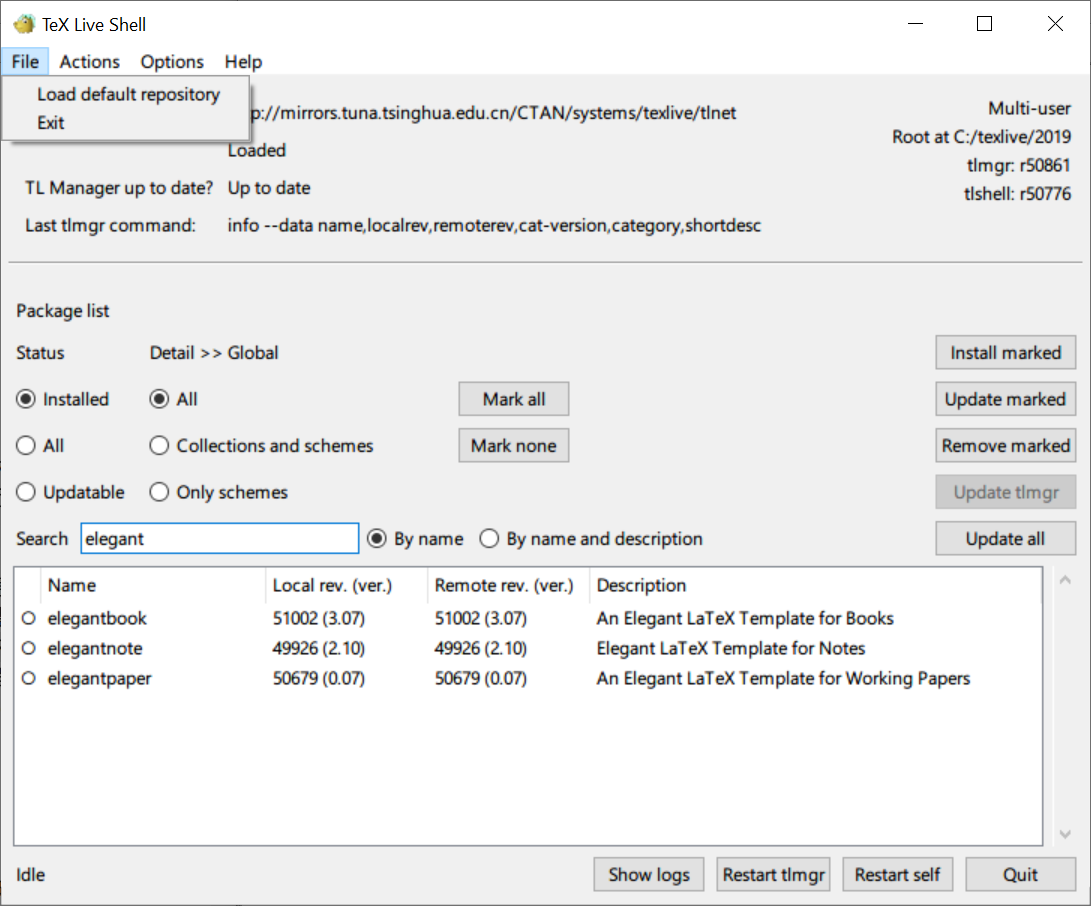
\includegraphics[width=0.7\textwidth]{tlshell.png}
	\caption{使用 \TeX{} Live Shell 安装 ElegantBook 模板}
	\end{figure}
	
	如果你是 \TeX{} Live 2018 的用户,由于 2018 无法直接更新到 2019,所以你想更新的话,需要卸载 2018 重装 2019。如果你实在不想折腾,那么你仍然可以使用本模板。你可以手动安装模板,将 \lstinline{elegantbook.cls} 复制到你的 \TeX{} Live 目录下,默认安装目录为 \lstinline|C:\texlive\2019\texmf-dist\tex\latex\elegantbook|,然后通过命令行(管理员权限),运行 \lstinline{texhash} 即可。
	
	啥?你是 C\TeX{} 用户?Sorry,本模板不提供支持。
	
	更多关于 \TeX{} Live 2019 的安装使用以及 C\TeX{} 与 \TeX{} Live 的兼容、系统路径问题,请参考官方文档以及啸行的\href{https://github.com/OsbertWang/install_latex/releases}{一份简短的安装 \LaTeX{} 的介绍}。
	
	\section{在线使用模板}
	考虑到用户的在线合作需求,我们把三套模板全部上传到 \href{https://www.overleaf.com/}{Overleaf} 上了,网络通畅的用户可以直接通过 Overleaf 在线使用我们的模板。这样的好处是无需安装 \TeX{} Live 2019,可以随时随地访问自己的文件。查找模板,请在 Overleaf 模板库里面搜索 \lstinline{elegantlatex} 即可,你也可以直接访问\href{https://www.overleaf.com/latex/templates?addsearch=elegantlatex}{搜索结果}。选择适当的模板之后,将其 \lstinline{Open as Template},即可把模板存到自己账户下,然后可以自由编辑以及与别人一起协作。更多关于 Overleaf 的介绍和使用,请参考 Overleaf 的\href{https://www.overleaf.com/learn}{官方文档}。
	
	\begin{remark}
	Overleaf 上,中文需要使用 \lstinline{XeLaTeX} 进行编译,英文可以使用 \lstinline{PDFLaTeX} 与 \lstinline{XeLaTeX} 进行编译。
	\end{remark}
	
	\section{用户作品计划}
	Elegant\LaTeX{} 系列模板从创立至今已经有 8 年了,我们的模板也受到了很多用户的喜爱,在此,为了促进模板用户之间的交流,了解用户需求,完善本模板,我们将建立一个区域专门展示用户的文档,包括但不限于 Github 和官网等。如果你愿意将自己的作品展示出来,请邮件或者其他方式联系我们。如果自己代码已经传到 Github 或者 Gitee 等网站,可以提供对应网址。
	
	\section{关于提交}
	出于某些因素的考虑,Elegant\LaTeX{} 项目自 2019 年 5 月 20 日开始,\textbf{不再接受任何非作者预约性质的提交}(pull request)!如果你想改进模板,你可以给我们提交 issues,或者可以在遵循协议(LPPL-1.3c)的情况下,克隆到自己仓库下进行修改。
	
	\section{协作人员招募}
	招募 Elegant\LaTeX{} 的协作人员,没有工资。工作内容:翻译 Elegant\LaTeX{} 系列模板相关的文稿(中文->英文),维护模板的 wiki(主要涉及 Markdown 语法),如果有公众号文稿写作经历的话,也可以帮忙写微信稿。本公告长期有效。
	
	\section{致谢}
	2019 年 5 月 20 日,ElegantBook 模板在 Github 上的 star 数达到了 100,并且 21 日上了 Github 网站 \TeX{} 语言的\href{https://github.com/trending/tex?since=daily}{日趋势榜单}。这对于 Elegant\LaTeX{} 系列模板都是一个里程碑!
	
	在此特别感谢 China\TeX{} 以及 \href{http://www.latexstudio.net/}{\LaTeX{} 工作室}对于本系列模板的大力宣传与推广。\LaTeX{} 工作室网站上有很多精彩的帖子和精致的模板,欢迎大家去挖掘里面的宝藏。这也是国内最全面的 \LaTeX{} 相关的网站。
	
	特别感谢 \href{https://github.com/muzimuzhi}{muzimuzhi} 对于模板的完善。
	
	如果你喜欢我们的模板,你可以在 Github 上收藏我们的模板。
	\begin{figure}[htbp]
	\centering
	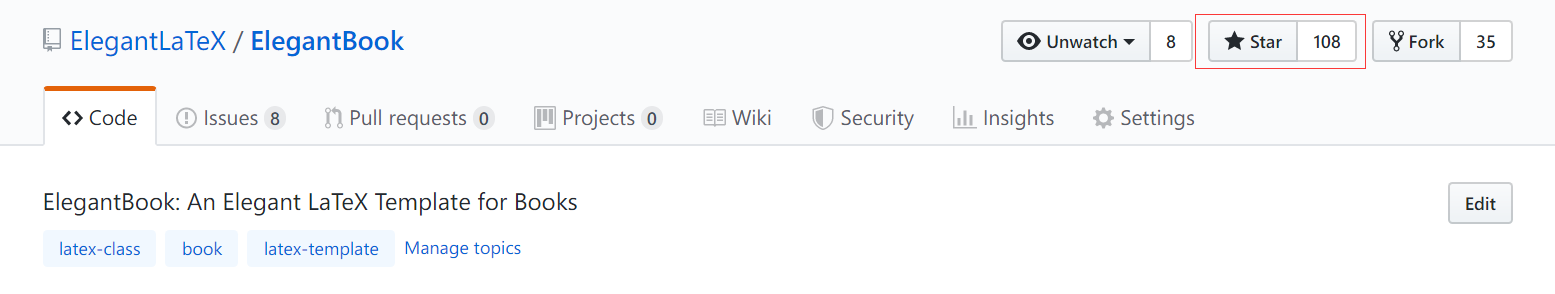
\includegraphics[width=\textwidth]{star.png}
	\caption{一键三连求赞}
	\end{figure}
	
	之前我们模板从未发布过捐赠/打赏信息,近期有用户反映他们对我们模板非常喜爱,想打赏没有支付码,不禁感叹,这世道变了啊,还有主动打赏的,那么我们就“勉为其难”地发布我们的打赏二维码吧!
	
	\begin{figure}[htbp]
	\centering
	
\includegraphics[width=0.5\textwidth]{donate.jpg}
	\end{figure}
	
	赞赏费用的使用解释权归 Elegant\LaTeX{} 所有,并且不接受监督,请自愿理性打赏,10 元以上的赞赏,我们将列入捐赠榜,谢谢各位金主!
	
	\begin{table}[htbp]
 \centering
 \caption{捐赠榜}
  \begin{tabular}{crcc}
  \toprule
  捐赠者   & 金额 & 时间 & 渠道 \\
  \midrule
  Lerh  & 10 元  & 2019/05/15 & 微信 \\
  越过地平线 & 10 元    & 2019/05/15 & 微信 \\
		大熊 &  20 元 & 2019/05/27 & 微信 \\
		佚名 & 10 元 & 2019/05/30 & 微信\\
		\href{http://www.latexstudio.net/}{latexstudio.net} & 666 元 & 2019/06/05 & 支付宝\\
  \bottomrule
  \end{tabular}%
	\end{table}%
	
	再次感谢大家对于模板的喜爱!
	
	\chapter{ElegantBook 设置说明}
	本模板基于基础的 book 文类,所以 book 的选项对于本模板也是有效的。默认编码为 UTF-8,推荐使用 \TeX{} Live 编译。本文编写环境为 Win10 (64bit) + \TeX{} Live 2019,支持 \lstinline{PDFLaTeX} 以及 \lstinline{XeLaTeX} 编译。
	
	
	\section{语言模式}
	本模板内含两套语言环境,改变语言环境会改变图表标题的引导词(图,表),文章结构词(比如目录,参考文献等),以及定理环境中的引导词(比如定理,引理等)。不同语言模式的启用如下:
	\begin{lstlisting}
	\documentclass[cn]{elegantbook} 
	\documentclass[lang=cn]{elegantbook}
	\end{lstlisting}
	
	\begin{remark}
	只有中文环境(\lstinline{lang=cn})才可以输入中文。另外如果抄录环境(\lstinline{lstlisting})中有中文字符,请务必使用 \lstinline{XeLaTeX} 编译。
	\end{remark}
	
	\section{设备选项}
	最早我们在 ElegantNote 模板中加入了设备选项(\lstinline{device}),后来,我们觉得这个设备选项的设置可以应用到 ElegantBook 中\footnote{不过因为 ElegantBook 模板封面图片的存在,在修改页面设计时,需要对图片进行裁剪。},而且 Book 一般内容比较多,如果在 iPad 上看无需切边,放大,那用户的阅读体验将会得到巨大提升。你可以使用下面的选项将版面设置为 iPad 设备模式\footnote{默认为 normal 模式,也即 A4 纸张大小。}
	\begin{lstlisting}
	\documentclass[pad]{elegantbook} %or
	\documentclass[device=pad]{elegantbook}
	\end{lstlisting}
	
	\section{颜色主题}
	本模板内置 5 组颜色主题,分别为 \textcolor{structure1}{\lstinline{green}}\footnote{为原先默认主题。}、\textcolor{structure2}{\lstinline{cyan}}、\textcolor{structure3}{\lstinline{blue}}(默认)、\textcolor{structure4}{\lstinline{gray}}、\textcolor{structure5}{\lstinline{black}}。另外还有一个自定义的选项  \lstinline{nocolor}。调用颜色主题 \lstinline{green} 的方法为 
	\begin{lstlisting}
	\documentclass[green]{elegantbook} %or
	\documentclass[color=green]{elegantbook}
	\end{lstlisting}
	
	\begin{table}[htbp]
	\caption{ElegantBook 模板中的颜色主题\label{tab:color thm}}
	\centering
	\begin{tabular}{ccccccc}
	\toprule
       & \textcolor{structure1}{green} 
       & \textcolor{structure2}{cyan} 
       & \textcolor{structure3}{blue}
       & \textcolor{structure4}{gray} 
       & \textcolor{structure5}{black} 
       & 主要使用的环境\\
	\midrule
	structure & \makecell{{\color{structure1}\rule{1cm}{1cm}}}
					& \makecell{{\color{structure2}\rule{1cm}{1cm}}}
					& \makecell{{\color{structure3}\rule{1cm}{1cm}}} 
					& \makecell{{\color{structure4}\rule{1cm}{1cm}}} 
					& \makecell{{\color{structure5}\rule{1cm}{1cm}}} 
					& chapter \ section \ subsection \\
	
	main      & \makecell{{\color{main1}\rule{1cm}{1cm}}}
					& \makecell{{\color{main2}\rule{1cm}{1cm}}}
					& \makecell{{\color{main3}\rule{1cm}{1cm}}}
					& \makecell{{\color{main4}\rule{1cm}{1cm}}}
					& \makecell{{\color{main5}\rule{1cm}{1cm}}}
					& definition \ exercise \ problem \\
	
	second    & \makecell{{\color{second1}\rule{1cm}{1cm}}}
					& \makecell{{\color{second2}\rule{1cm}{1cm}}}
					& \makecell{{\color{second3}\rule{1cm}{1cm}}}
					& \makecell{{\color{second4}\rule{1cm}{1cm}}}
					& \makecell{{\color{second5}\rule{1cm}{1cm}}}
					& theorem \ lemma \ corollary\\
	
	third     & \makecell{{\color{third1}\rule{1cm}{1cm}}}
					& \makecell{{\color{third2}\rule{1cm}{1cm}}}
					& \makecell{{\color{third3}\rule{1cm}{1cm}}}
					& \makecell{{\color{third4}\rule{1cm}{1cm}}}
					& \makecell{{\color{third5}\rule{1cm}{1cm}}}
					& proposition\\
	\bottomrule
	\end{tabular}
	\end{table}
	
	如果需要自定义颜色的话请选择 \lstinline{nocolor} 选项或者使用 \lstinline{color=none},然后在导言区定义 structurecolor、main、second、third 颜色,具体方法如下:
	\begin{lstlisting}
	\definecolor{structurecolor}{RGB}{0,0,0}
	\definecolor{main}{RGB}{70,70,70}    
	\definecolor{second}{RGB}{115,45,2}    
	\definecolor{third}{RGB}{0,80,80}   
	\end{lstlisting}
	
	
	\section{章标题显示风格}
	
	本模板内置 2 套\textit{章标题显示风格},包含 \lstinline{hang}(默认)与 \lstinline{display} 两种风格,区别在于章标题单行显示(\lstinline{hang})与双行显示(\lstinline{display}),本说明使用了 \lstinline{hang}。调用方式为
	\begin{lstlisting}
	\documentclass[hang]{elegantbook} %or
	\documentclass[titlestyle=hang]{elegantbook}
	\end{lstlisting}
	
	\section{数学环境简介}
	
	在我们这个模板中,我们定义了两种不同的定理模式 \lstinline{mode},包括简单模式(\lstinline{simple})和炫彩模式(\lstinline{fancy}),默认为 \lstinline{fancy} 模式,不同模式的选择为
	\begin{lstlisting}
	\documentclass[simple]{elegantbook} %or
	\documentclass[mode=simple]{elegantbook}
	\end{lstlisting}
	
	本模板定义了四大类环境
	
	\begin{itemize}
	\item \textit{定理类环境},包含标题和内容两部分,全部定理类环境的编号均以章节编号。根据格式的不同分为 3 种
 \begin{itemize}
    \item \textcolor{main}{\textbf{definition}} 环境,颜色为 \textcolor{main}{main};
    \item \textcolor{second}{\textbf{theorem、lemma、corollary}} 环境,颜色为 \textcolor{second} {second};
    \item \textcolor{third}{\textbf{proposition}} 环境,颜色为 \textcolor{third}{third}。
 \end{itemize}
	\item \textit{示例类环境},有 \textbf{example、exercise、problem} 环境(对应于例,练习,例题),自动编号,编号以章节为单位。
	\item \textit{证明类环境},有 \textbf{proof、note} 环境,特点是,有引导符或者结尾符,\textbf{note} 环境有引导符号,\textbf{proof} 环境有证明完毕符号。
	\item \textit{结论类环境},有 \textbf{conclusion、assumption、property,remark、solution} 环境\footnote{本模板还添加了一个 result 选项,用于隐藏 \lstinline{solution} 和 \lstinline{proof} 环境,默认为显示(\lstinline{result=answer}),隐藏使用 \lstinline{result=noanswer}。},三者均以粗体的引导词为开头,和普通段落格式一致。
	\end{itemize}
	
	\subsection{定理类环境的使用}
	由于本模板使用了 \lstinline{tcolorbox} 宏包来定制定理类环境,所以和普通的定理环境的使用有些许区别,定理的使用方法如下:
	\begin{lstlisting}
	\begin{theorem}{theorem name}{label}
	The content of theorem.
	\end{theorem}
	\end{lstlisting}
	
	第一个必选项 \lstinline{theorem name} 是定理的名字,第二个必选项 \lstinline{label} 是交叉引用时所用到的标签,交叉引用的方法为 \verb|\ref{thm:label}|。请注意,交叉引用时必须加上前缀 \lstinline{thm:}。
	
	其他相同用法的定理类环境有:
	
	\begin{table}[htbp]
 \centering
 \caption{定理类环境}
   \begin{tabular}{llll}
   \toprule
   环境名 & 标签名 & 前缀 & 交叉引用 \\
   \midrule
   definition & label & def   & \lstinline|\ref{def:label}| \\
   theorem & label & thm   & \lstinline|\ref{thm:label}| \\
   lemma & label & lem   & \lstinline|\ref{lem:label}| \\
   corollary & label & cor   & \lstinline|\ref{cor:label}| \\
   proposition & label & pro   & \lstinline|\ref{pro:label}| \\
   \bottomrule
   \end{tabular}%
 \label{tab:theorem-class}%
 \end{table}%
 
	
	\subsection{其他环境的使用}
	其他三种环境没有选项,可以直接使用,比如 \lstinline{example} 环境的使用方法与效果:
	\begin{lstlisting}
	\begin{example}
 This is the content of example environment.
	\end{example}
	\end{lstlisting}
	
	\begin{example}
	This is the content of example environment.
	\end{example}
	
	
	这几个都是同一类环境,区别在于
	
	\begin{itemize}
 \item 示例环境(example)、练习(exercise)与例题(problem)章节自动编号;
 \item 注意(note)环境有提醒引导符,证明(proof)环境有证明结束符;
 \item 结论(conclusion)等环境都是普通段落环境,引导词加粗。
	\end{itemize}
	
	\section{装饰物}
	
	本模板为章节后的装饰物(base)添加了隐藏选项,有 \lstinline{show} 和 \lstinline{hide} 两个选项。
	\begin{lstlisting}
	\documentclass[hide]{elegantbook} %or
	\documentclass[base=hide]{elegantbook}
	\end{lstlisting}
	
	\section{封面和徽标}
	
	本模板使用的封面图片来源于 \href{https://pixabay.com/en/tea-time-poetry-coffee-reading-3240766/}{pixabay.com}\footnote{感谢 China\TeX{} 提供免费图源网站,另外还推荐 \href{https://www.pexels.com/}{pexels.com}。},图片完全免费,可用于任何场景。封面图片的尺寸为 $1280 \times 1024$, 更换图片的时候请\textbf{严格}按照封面图片尺寸进行裁剪。推荐一个免费的在线图片裁剪网站 \href{https://www.befunky.com/create/crop-photo/}{befunky.com}。
	
	本文用到的 Logo 比例为 1:1,也即正方形图片,在更换图片的时候请选择合适的图片进行替换。
	
	\section{列表环境}
	本模板借助于 \lstinline{tikz} 定制了 \lstinline{itemize} 和 \lstinline{enumerate} 环境,其中 \lstinline{itemize} 环境修改了 3 层嵌套,而 \lstinline{enumerate} 环境修改了 4 层嵌套(仅改变颜色)。示例如下\\[2ex]
	\begin{minipage}[b]{0.49\textwidth}
	\begin{itemize}
 \item first item of nesti;
 \item second item of nesti;
 \begin{itemize}
    \item first item of nestii;
    \item second item of nestii;
    \begin{itemize}
       \item first item of nestiii;
       \item second item of nestiii.
    \end{itemize}   
 \end{itemize}
	\end{itemize}
	\end{minipage}
	\begin{minipage}[b]{0.49\textwidth}
	\begin{enumerate}
 \item first item of nesti;
 \item second item of nesti;
 \begin{enumerate}
    \item first item of nestii;
    \item second item of nestii;
    \begin{enumerate}
       \item first item of nestiii;
       \item second item of nestiii.
    \end{enumerate}   
 \end{enumerate}
	\end{enumerate}
	\end{minipage}
	
	\section{参考文献}
	
	此模板使用了 \hologo{BibTeX} 来生成参考文献,在中文示例中,使用了 \lstinline{gbt7714} 宏包。参考文献示例:\cite{en1,en2,en3} 使用了中国一个大型的 P2P 平台(人人贷)的数据来检验男性投资者和女性投资者在投资表现上是否有显著差异。
	
	你可以在谷歌学术,Mendeley,Endnote 中获得文献条目(bib item),然后把它们添加到 \lstinline{reference.bib} 中。在文中引用的时候,引用它们的键值(bib key)即可。注意需要在编译的过程中添加 \hologo{BibTeX} 编译。如果你想添加未引用的文献,可以使用
	\begin{lstlisting}[frame=single]
	\nocite{EINAV2010,Havrylchyk2018} %or include some bibitems
	\nocite{*} %include all the bibitems
	\end{lstlisting}
	
	本模板还添加了 \lstinline{cite=numbers} 和 \lstinline{cite=authoryear} 两个参考文献选项,用于设置参考文献格式的设置,默认为 \lstinline{numbers}。据我们所知,理工科类一般使用 \lstinline{numbers},而文科类使用 \lstinline{authoryear} 比较多,所以我们将 \lstinline{numbers} 作为默认格式。如果需要改为  \lstinline{authoryear} ,可以使用
	\begin{lstlisting}
	\documentclass[cite=authoryear]{elegantbook} %or
	\documentclass[authoryear]{elegantbook}
	\end{lstlisting}
	
	\section{添加序章}
	
	如果你想在第一章前面添序章,不改变原本章节序号,可以在第一章内容前面使用 
	\begin{lstlisting}
	\chapter*{Introduction}
	\addcontentsline{toc}{chapter}{Introduction} 
	\markboth{Introduction}{} 
	The content of introduction.
	\end{lstlisting}
	
	\section{章节摘要}
	模板新增了一个章节摘要环境(introduction),使用示例
	\begin{lstlisting}
	\begin{introduction}
		\item Definition of Theorem
		\item Ask for help
		\item Optimization Problem
		\item Property of Cauchy Series
		\item Angle of Corner
	\end{introduction}
	\end{lstlisting}
	效果如下:
	\begin{introduction}
		\item Definition of Theorem
		\item Ask for help
		\item Optimization Problem
		\item Property of Cauchy Series
		\item Angle of Corner
	\end{introduction}
	
	环境的标题文字可以通过这个环境的可选参数进行修改,修改方法为:
	\begin{lstlisting}
	\begin{introduction}[Brief Introduction]
	...
	\end{introduction}
	\end{lstlisting}
	
	
	\section{章后习题}
	前面我们介绍了例题和练习两个环境,这里我们再加一个,章后习题(\lstinline{problemset})环境,用于在每一章结尾,显示本章的练习。使用方法如下
	
	\begin{lstlisting}
	\begin{problemset}
		\item exercise 1
		\item exercise 2
		\item exercise 3
	\end{problemset}
	\end{lstlisting}
	
	
	效果如下:
	\begin{problemset}
		\item exercise 1
		\item exercise 2
		\item exercise 3
	\end{problemset}
	
	\begin{remark}
	如果你想把 \lstinline{problemset} 环境的标题改为其他文字,你可以类似于 introduction 环境修改 problemset 的可选参数。
	\end{remark}
	
	\chapter{ElegantBook 写作示例}
	
	\begin{introduction}
	\item 积分定义~\ref{def:int}
	\item Fubini 定理~\ref{thm:fubi}
	\item 最优性原理~\ref{pro:max}
	\item 柯西列性质~\ref{property:cauchy}
	\item 韦达定理
	\end{introduction}
	
	\section{Lebesgue 积分}
	在前面各章做了必要的准备后,本章开始介绍新的积分。在 Lebesgue 测度理论的基础上建立了 Lebesgue 积分,其被积函数和积分域更一般,可以对有界函数和无界函数统一处理。正是由于 Lebesgue 积分的这些特点,使得 Lebesgue 积分比 Riemann 积分具有在更一般条件下的极限定理和累次积分交换积分顺序的定理,这使得 Lebesgue 积分不仅在理论上更完善,而且在计算上更灵活有效。
	
	Lebesgue 积分有几种不同的定义方式。我们将采用逐步定义非负简单函数,非负可测函数和一般可测函数积分的方式。
	
	由于现代数学的许多分支如概率论、泛函分析、调和分析等常常用到一般空间上的测度与积分理论,在本章最后一节将介绍一般的测度空间上的积分。
	
	\subsection{积分的定义}
	
	我们将通过三个步骤定义可测函数的积分。首先定义非负简单函数的积分。以下设 $E$ 是 $\mathcal{R}^n$ 中的可测集。
	
	\begin{itemize}
	\item 名词解释
	\begin{definition}{可积性}{int}
	设 $ f(x)=\sum\limits_{i=1}^{k} a_i \chi_{A_i}(x)\oint_{a}^b\ointop_{a}^b\prod_{i=1}^n$ 是 $E$ 上的非负简单函数,其中 $\{A_1,A_2,\ldots,A_k\}$ 是 $E$ 上的一个可测分割,$a_1,a_2,\ldots,a_k$ 是非负实数。定义 $f$ 在 $E$ 上的积分为 $\int_{a}^b f(x)$
	\begin{equation}
 \label{inter}
 \int_{E} f dx = \sum_{i=1}^k a_i m(A_i) \pi \alpha\beta\sigma\gamma\nu\xi\epsilon\varepsilon. \oint_{a}^b\ointop_{a}^b\prod_{i=1}^n
	\end{equation}
	一般情况下 $0 \leq \int_{E} f dx \leq \infty$。若 $\int_{E} f dx < \infty$,则称 $f$ 在 $E$ 上可积。
	\end{definition}
	\item 测试 2
	\end{itemize}
	
	
	
	一个自然的问题是,Lebesgue 积分与我们所熟悉的 Riemann 积分有什么联系和区别?在 4.4 在我们将详细讨论 Riemann 积分与 Lebesgue 积分的关系。这里只看一个简单的例子。设 $D(x)$ 是区间 $[0,1]$ 上的 Dirichlet 函数。即 $D(x)=\chi_{Q_0}(x)$,其中 $Q_0$ 表示 $[0,1]$ 中的有理数的全体。根据非负简单函数积分的定义,$D(x)$ 在 $[0,1]$ 上的 Lebesgue 积分为
	\begin{equation}
 \label{inter2}
 \int_0^1 D(x)dx = \int_0^1 \chi_{Q_0} (x) dx = m(Q_0) = 0
	\end{equation}
	即 $D(x)$ 在 $[0,1]$ 上是 Lebesgue 可积的并且积分值为零。但 $D(x)$ 在 $[0,1]$ 上不是 Riemann 可积的。
	
	
	
	有界变差函数是与单调函数有密切联系的一类函数。有界变差函数可以表示为两个单调递增函数之差。与单调函数一样,有界变差函数几乎处处可导。与单调函数不同,有界变差函数类对线性运算是封闭的,它们构成一线空间。练习题 \ref{exer:43} 是一个性质的证明。
	
	\begin{exercise}\label{exer:43}
	设 $f \notin\in L(\mathcal{R}^1)$,$g$ 是 $\mathcal{R}^1$ 上的有界可测函数。证明函数
	\begin{equation}
 \label{ex:1}
 I(t) = \int_{\mathcal{R}^1} f(x+t)g(x)dx \quad t \in \mathcal{R}^1
	\end{equation}
	是 $\mathcal{R}^1$ 上的连续函数。
	\end{exercise}
	
	\begin{problem}
	即 $D(x)$ 在 $[0,1]$ 上是 Lebesgue 可积的并且积分值为零。但 $D(x)$ 在 $[0,1]$ 上不是 Riemann 可积的。
	\end{problem}
	
	\begin{example}
	即 $D(x)$ 在 $[0,1]$ 上是 Lebesgue 可积的并且积分值为零。但 $D(x)$ 在 $[0,1]$ 上不是 Riemann 可积的。
	\end{example}
	
	\begin{solution}
	即 $D(x)$ 在 $[0,1]$ 上是 Lebesgue 可积的并且积分值为零。但 $D(x)$ 在 $[0,1]$ 上不是 Riemann 可积的。
	\end{solution}
	
	\begin{theorem}{Fubini 定理}{fubi} 
	(1)若 $f(x,y)$ 是 $\mathcal{R}^p\times\mathcal{R}^q$ 上的非负可测函数,则对几乎处处的 $x\in \mathcal{R}^p$,$f(x,y)$ 作为 $y$ 的函数是 $\mathcal{R}^q$ 上的非负可测函数,$g(x)=\int_{\mathcal{R}^q}f(x,y) dy$ 是 $\mathcal{R}^p$ 上的非负可测函数。并且
	\begin{equation}
 \label{eq:461}
 \int_{\mathcal{R}^p\times\mathcal{R}^q} f(x,y) dxdy=\int_{\mathcal{R}^p}\left(\int_{\mathcal{R}^q}f(x,y)dy\right)dx.
	\end{equation}
	(2)若 $f(x,y)$ 是 $\mathcal{R}^p\times\mathcal{R}^q$ 上的可积函数,则对几乎处处的 $x\in\mathcal{R}^p$,$f(x,y)$ 作为 $y$ 的函数是 $\mathcal{R}^q$ 上的可积函数,并且 $g(x)=\int_{\mathcal{R}^q}f(x,y) dy$ 是 $\mathcal{R}^p$ 上的可积函数。而且~\ref{eq:461} 成立。
	\end{theorem}
	
	\begin{note}
	在本模板中,引理(lemma),推论(corollary)的样式和定理~\ref{thm:fubi} 的样式一致,包括颜色,仅仅只有计数器的设置不一样。
	\end{note}
	
	我们说一个实变或者复变量的实值或者复值函数是在区间上平方可积的,如果其绝对值的平方在该区间上的积分是有限的。所有在勒贝格积分意义下平方可积的可测函数构成一个希尔伯特空间,也就是所谓的 $L^2$ 空间,几乎处处相等的函数归为同一等价类。形式上,$L^2$ 是平方可积函数的空间和几乎处处为 0 的函数空间的商空间。
	
	\begin{proposition}{最优性原理}{max}
	如果 $u^*$ 在 $[s,T]$ 上为最优解,则 $u^*$ 在 $[s, T]$ 任意子区间都是最优解,假设区间为 $[t_0, t_1]$ 的最优解为 $u^*$ ,则 $u(t_0)=u^{*}(t_0)$,即初始条件必须还是在 $u^*$ 上。
	\end{proposition}
	
	我们知道最小二乘法可以用来处理一组数据,可以从一组测定的数据中寻求变量之间的依赖关系,这种函数关系称为经验公式。本课题将介绍最小二乘法的精确定义及如何寻求点与点之间近似成线性关系时的经验公式。假定实验测得变量之间的 $n$ 个数据,则在平面上,可以得到 $n$ 个点,这种图形称为 “散点图”,从图中可以粗略看出这些点大致散落在某直线近旁, 我们认为其近似为一线性函数,下面介绍求解步骤。
	
	\begin{figure}[htbp]
		\centering
		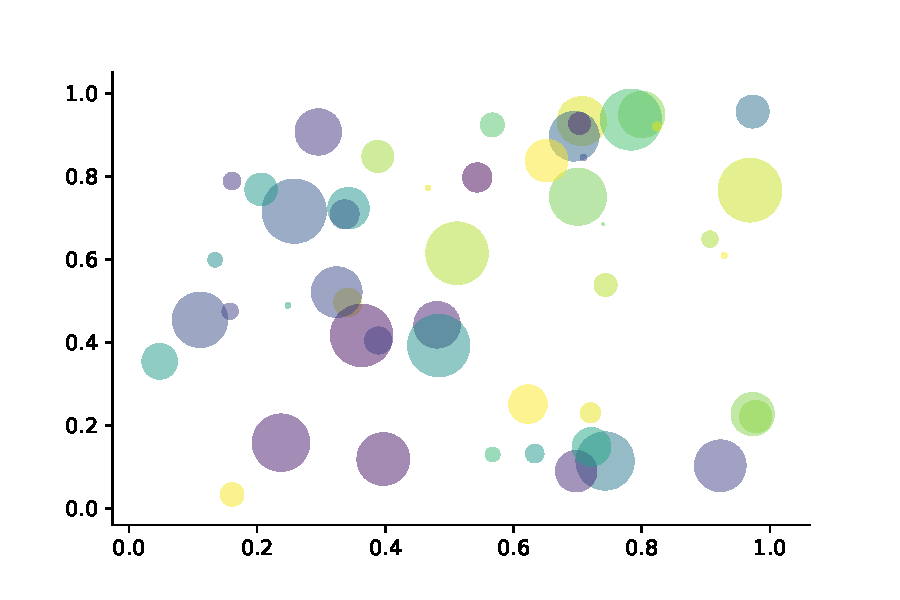
\includegraphics[width=0.6\textwidth]{scatter.pdf}
		\caption{散点图示例 $\hat{y}=a+bx$ \label{fig:scatter}}
	\end{figure}
	
	以最简单的一元线性模型来解释最小二乘法。什么是一元线性模型呢?监督学习中,如果预测的变量是离散的,我们称其为分类(如决策树,支持向量机等),如果预测的变量是连续的,我们称其为回归。回归分析中,如果只包括一个自变量和一个因变量,且二者的关系可用一条直线近似表示,这种回归分析称为一元线性回归分析。如果回归分析中包括两个或两个以上的自变量,且因变量和自变量之间是线性关系,则称为多元线性回归分析。对于二维空间线性是一条直线;对于三维空间线性是一个平面,对于多维空间线性是一个超平面。
	
	\begin{property}\label{property:cauchy}
	柯西列的性质
	\begin{enumerate}
	\item $\{x_k\}$ 是柯西列,则其子列 $\{x_k^i\}$ 也是柯西列。
	\item $x_k\in \mathcal{R}^n$,$\rho(x,y)$ 是欧几里得空间,则柯西列收敛,$(\mathcal{R}^n,\rho)$ 空间是完备的。
	\end{enumerate}
	\end{property}
	
	\begin{conclusion}
	回归分析(regression analysis) 是确定两种或两种以上变量间相互依赖的定量关系的一种统计分析方法。运用十分广泛,回归分析按照涉及的变量的多少,分为一元回归和多元回归分析;按照因变量的多少,可分为简单回归分析和多重回归分析;按照自变量和因变量之间的关系类型,可分为线性回归分析和非线性回归分析。
	\end{conclusion}
	
	\begin{problemset}
	\item 设 $A$ 为数域 $K$ 上的 $n$ 级矩阵。证明:如果 $K^n$ 中任意非零列向量都是 $A$ 的特征向量,则 $A$ 一定是数量矩阵。
	\item 证明:不为零矩阵的幂零矩阵不能对角化。
	\item 设 $A = (a_{ij})$ 是数域 $K$ 上的一个 $n$ 级上三角矩阵,证明:如果 $a_{11} = a_{22} = \cdots = a_{nn}$,并且至少有一个 $a_{kl} \not = 0 (k < l)$,则 $A$ 一定不能对角化。
	\end{problemset}
	
	\chapter{旁注}
	在 3.08 版本,我们加入了旁注(边注)等设置以及 \lstinline{\elegantpar} 命令,不过目前处于测试阶段。如果你想整个文档都加入旁注,一般的方法是,重新设置旁注的大小。本模板加入了一个旁注选项 \lstinline{marginpar},如果加入旁注 \lstinline{marginpar=margintrue},则会减少版芯两边的宽度(减少至 1.5cm),如果不加入旁注 \lstinline{marginpar=marginfalse}(默认),则维持两边距离不变。旁注选项仅对 \lstinline{device=normal} 试用,pad 模式并不支持。
	
	旁注命令可以使用 \LaTeX{} 自带的 \lstinline{\marginpar} 命令或者 \lstinline{marginnote}  宏包的  \lstinline{\marginnote}  命令,旁注的使用,请参考维基百科:\href{https://en.wikibooks.org/wiki/LaTeX/Footnotes_and_Margin_Notes#Margin_Notes}{旁注}或者 \LaTeX {}书籍。
	
	本模板还添加了一个 \lstinline{\elegantpar} 命令,需要注意的是,由于这个命令使用了 TikZ 中的层叠效果(overlay),所以为了得到正确的旁注显示,你需要多次编译(3 次)。\lstinline{\elegantpar} 命令的效果如下。
	
	%\setlength{\marginparwidth}{2.5cm}
	Lorem ipsum dolor sit amet, consectetur adipisicing elit, sed do eiusmod
	tempor incididunt ut labore et \elegantpar{dolore magna aliqua}{This is Beautiful the elegantpar Style for English Text}. Ut enim ad minim veniam,
	quis nostrud exercitation ullamco laboris nisi ut aliquip ex ea commodo
	consequat. Duis aute irure dolor in reprehenderit in voluptate velit esse
	cillum dolore eu fugiat nulla pariatur. Excepteur sint occaecat cupidatat non
	proident, sunt in culpa qui officia deserunt mollit anim id est laborum.
	
	\begin{equation}
	a^{2}+b^{2} = \elegantpar{c^{2}}{勾股定理
	\begin{equation*}a^2+b^2=c^2\end{equation*}}
	\end{equation}
 
 若夫日出而林霏开,云归而岩穴暝,晦明变化者,山间之朝暮也。野芳发而幽香,佳木秀而繁阴,风霜高洁,水落而石出者,山间之四时也。朝而往,暮而归,四时之景不同,而乐亦无穷也。 
 
 至于负者歌于途,行者休于树,前者呼,后者应,\elegantpar{伛偻提携}{指搀扶着走的小孩子},往来而不绝者,滁人游也。临溪而渔,溪深而鱼肥。酿泉为酒,泉香而酒洌;山肴野蔌,杂然而前陈者,太守宴也。宴酣之乐,非丝非竹,射者中,弈者胜,觥筹交错,起坐而喧哗者,众宾欢也。苍颜白发,颓然乎其间者,太守醉也。$2\elegantpar{x}{方程的解与数学符号的选择无关}=3$。
	
	\chapterno{常见问题集}
	
	\begin{custom}{问题}
	有没有办法章节用“第一章,第一节,(一)”这种?
	\end{custom}
	
	\begin{solution}
	你可以修改模板中对于章节的设置,利用 ctex 宏集的 \lstinline{\zhnumber} 命令可以把计数器的数字形式转为中文。
	\end{solution}
	
	
	\begin{custom}{问题}
	3.07 版本的 cls 的 natbib 加了numbers 编译完了没变化,群主设置了不可更改了?
	\end{custom}
	
	\begin{solution}
	3.07 中在 \lstinline{gbt7714} 宏包使用时,加入了 \lstinline{authoryear} 选项,这个使得 \lstinline{natbib} 设置了 \lstinline{numbers} 也无法生效。3.08 版本中,模板增加了 \lstinline{numbers} 和 \lstinline{authoryear} 文献选项,你可以参考前文设置说明。
	\end{solution}
	
	\begin{custom}{问题}
	大佬,我想把正文字体改为亮色,背景色改为黑灰色。
	\end{custom}
	
	\begin{solution}
	页面颜色可以使用 \lstinline{\pagecolor} 命令设置,文本命令可以参考\href{https://tex.stackexchange.com/questions/278544/xcolor-what-is-the-equivalent-of-default-text-color}{这里}进行设置。
	\end{solution}
	
	\begin{custom}{问题}
	\lstinline{! LaTeX Error: Unknown option `scheme=plain' for package `ctex'.}
	\end{custom}
	
	\begin{solution}
	你用的 C\TeX{} 套装吧?这个里面的 \lstinline{ctex} 宏包已经是已经是 10 年前的了,与本模板使用的 \lstinline{ctex} 宏集有很大区别。不建议 C\TeX{} 套装了,请卸载并安装 \TeX{} Live 2019。
	\end{solution}
	
	\begin{custom}{问题}
	我该使用什么版本?
	\end{custom}
	
	\begin{solution}
	请务必使用\href{https://github.com/ElegantLaTeX/ElegantBook/releases}{最新正式发行版},发行版间不定期可能会有更新(修复 bug 或者改进之类),如果你在使用过程中没有遇到问题,不需要每次更新\href{https://github.com/ElegantLaTeX/ElegantBook/archive/master.zip}{最新版},但是在发行版更新之后,请尽可能使用最新版(发行版)!最新发行版可以在 Github 或者 \TeX{} Live 2019 内获取。
	\end{solution}
	
	
	\begin{custom}{问题}
	我该使用什么编辑器?
	\end{custom}
	
	\begin{solution}
	你可以使用 \TeX{} Live 2019 自带的编辑器 \TeX{}works 或者使用 \TeX{}studio,\TeX works 的自动补全,你可以参考我们的总结 \href{https://github.com/EthanDeng/texworks-autocomplete}{\TeX works 自动补全}。推荐使用 \TeX{} Live 2019 + \TeX Studio。我自己用 VS Code 和 Sublime Text,相关的配置说明,请参考 \href{https://github.com/EthanDeng/vscode-latex}{\LaTeX{} 编译环境配置:Visual Studio Code 配置简介} 和 \href{https://github.com/EthanDeng/sublime-text-latex}{Sublime Text 搭建 \LaTeX{} 编写环境}。
	\end{solution}
	
	
	\begin{custom}{问题}
	您好,我们想用您的 ElegantBook 模板写一本书。关于机器学习的教材,希望获得您的授权,谢谢您的宝贵时间。
	\end{custom}
	
	\begin{solution}
	模板的使用修改都是自由的,你们声明模板来源以及模板地址(github 地址)即可,其他未尽事宜按照开源协议 LPPL-1.3c。做好之后,如果方便的话,可以给我们一个链接,我把你们的教材放在 ElegantLaTeX 用户作品集里。
	\end{solution}
	
	\begin{custom}{问题}
	我想要原来的封面!
	\end{custom}
	
	\begin{solution}
	我们计划在未来版本加入封面选择,让用户可以选择旧版封面。
	\end{solution}
	
	\begin{custom}{问题}
	我想修改中文字体!
	\end{custom}
	
	\begin{solution}
	首先,我们{\heiti 强烈建议你不要去修改字体}!如果你一定坚持修改字体,请在 \lstinline{newtxtext} 宏包加载前加入中文字体设置(\lstinline{xeCJK} 宏包)。如果你选择自定义字体,请设置好 \lstinline{\kaishu},\lstinline{\heiti} 等命令,否则会报错。如果你看不懂我现在说的,请停止你的字体自定义行为。
	\end{solution}
	
	\begin{custom}{问题}
	请问交叉引用是什么?
	\end{custom}
	
	\begin{solution}
	本群和本模板适合有一定 \LaTeX{} 基础的用户使用,新手请先学习 \LaTeX{} 的基础,理解各种概念,否则你将寸步难行。
	\end{solution}
	
	\begin{custom}{问题}
	定义等环境中无法使用加粗命令么?
	\end{custom}
	
	\begin{solution}
	是这样的,默认中文并没加粗命令,如果你想在定义等环境中使用加粗命令,请使用 \lstinline{\heiti} 等字体命令,而不要使用 \lstinline{\textbf}。或者,你可以将 \lstinline{\textbf} 重新定义为 \lstinline{\heiti}。英文模式不存在这个问题。
	\end{solution}
	
	\begin{custom}{问题}
	代码高亮环境能用其他语言吗?
	\end{custom}
	
	\begin{solution}
	可以的,ElegantBook 模板用的是 \lstinline{listings} 宏包,你可以在环境之后加上语言,全局语言修改请使用 \lstinline{\lstset} 命令,更多信息请参考宏包文档。
	\end{solution}
	
	
	\begin{custom}{问题}
	群主,什么时候出 Beamer 的模板(主题),ElegantSlide 或者 ElegantBeamer?
	\end{custom}
	
	\begin{solution}
	这个问题问的人比较多,我这里给个明确的答案。由于 Beamer 中有一个很优秀的主题 \href{https://github.com/matze/mtheme}{Metropolis}。我觉得在我们找到非常好的创意之前不会发布正式的 Beamer 主题,如果你非常希望得到 Elegant\LaTeX{} “官方”的主题,请在用户 QQ 群内下载我们测试主题 PreElegantSlide(未来不一定按照这个制作)。正式版制作计划在 2020 年之后。
	\end{solution}
	
	\begin{custom}{问题}
	群主好棒,想嫁!
	\end{custom}
	
	\begin{solution}
	我取向正常!
	\end{solution}
	

	\nocite{*} 
	\addcontentsline{toc}{chapter}{参考文献}
	
	\bibliography{reference}
	

	\appendix
	
	\chapter{基本数学工具}
	
	本附录包括了计量经济学中用到的一些基本数学,我们扼要论述了求和算子的各种性质,研究了线性和某些非线性方程的性质,并复习了比例和百分数。我们还介绍了一些在应用计量经济学中常见的特殊函数,包括二次函数和自然对数,前 4 节只要求基本的代数技巧,第 5 节则对微分学进行了简要回顾;虽然要理解本书的大部分内容,微积分并非必需,但在一些章末附录和第 3 篇某些高深专题中,我们还是用到了微积分。
	
	\section{求和算子与描述统计量}
	
	\textbf{求和算子} 是用以表达多个数求和运算的一个缩略符号,它在统计学和计量经济学分析中扮演着重要作用。如果 $\{x_i: i=1, 2, \ldots, n\}$ 表示 $n$ 个数的一个序列,那么我们就把这 $n$ 个数的和写为:
	
	\begin{equation}
	\sum_{i=1}^n x_i \equiv x_1 + x_2 +\cdots + x_n
	\end{equation}
	
	\chapter{线性代数}
	
	\chapter{最小示例}
	
	\begin{lstlisting}
	\documentclass[lang=cn,11pt]{elegantbook}
	% title info
	\title{Title}
	\subtitle{Subtitle is here}
	% bio info
	\author{Your Name}
	\institute{XXX University}
	\date{\today}
	% extra info
	\version{1.00}
	\extrainfo{Victory won\rq t come to us unless we go to it. --- M. Moore}
	\logo{logo.png}
	\cover{cover.jpg}
	
	\begin{document}
	
	\maketitle
	\tableofcontents
	\mainmatter
	\hypersetup{pageanchor=true}
	% add preface chapter here if needed
	\chapter{Example Chapter Title}
	The content of chapter one.
	
	\bibliography{reference}
	
	\chapterno{索引}
	
	\end{document}
	\end{lstlisting}


\end{document}
